%PATH=/usr/local/texlive/2017/bin/x86_64-linux:$PATH
% The main file for my thesis
% each \textbf{chapter} is included from this main file
\documentclass[11pt,a4paper]{uolthesis}
%\documentclass[11pt,a4paper]{article}
%\usepackage{alltt,float}
%\usepackage{lgrind}
\usepackage{url}                    % for better handling of URL
\usepackage{lscape}                 % allow to use \begin{landscape}, which makes a page in landscape.
%\usepackage{subfigure}
\usepackage[T1]{fontenc}
\usepackage{mathrsfs}
\usepackage{graphicx}
%\usepackage{caption2}
%\usepackage{epstopdf}
%\usepackage{biblatex}[natbib]
%\usepackage{natbib}
%\usepackage[natbibapa]{apacite}
%\usepackage{natbib}
%\usepackage{biblatex}[natbib]
\usepackage{amsmath}
\usepackage{tikz}
\usepackage{pgfplots}
\usepackage{caption}
\usepackage{subcaption}
%\usepackage{pgfgantt}
\usepackage{multirow}
\usepackage{caption}
\usepackage{subcaption}
\usepackage{pgfplots}
\usepackage{tikz}
\usepackage[font=itshape]{quoting}
\usepackage{enumitem}
\usepackage{xr}
\usepackage[normalem]{ulem}
\usepackage{fancyhdr}
\usepackage{soul}
\externaldocument{ch2/Two}
\externaldocument{ch3/Three}
\externaldocument{ch3.5/ThreePointFive}
\externaldocument{ch4/Four}
\externaldocument{ch5/Five}
%\usepackage[maxnames=4,minnames=3,maxbibnames=99]{biblatex}
\usetikzlibrary{positioning}

\usetikzlibrary{shapes.arrows}

%\let\cite\shortcite

\newcommand{\citepos}[1]{\citeauthor{#1}'s \citeyearpar{#1}}
\newcommand{\citeposs}[1]{\citeauthor{#1}' \citeyearpar{#1}}
%\newcommand{\argmax}[1]{\underset{#1}{\operatorname{arg}\,\operatorname{max}}\;}
\newcommand{\del}[1]{\color{red}\sout{#1}\color{black}}
\newcommand{\rev}[1]{\color{blue}\uline{#1}\color{black}}
\newcommand{\revJB}[2]{\color{blue}JB-#1: \uline{#2}\color{black}}
\newcommand{\delJB}[1]{\color{red}JB: \sout{#1}\color{black}}
\newcommand{\revAK}[2]{\color{blue}AK-#1: \uline{#2}\color{black}}
\newcommand{\delAK}[1]{\color{red}AK: \sout{#1}\color{black}}
\newcommand{\revBO}[1]{\color{blue}JB/AK: #1\color{black}}
\newcommand{\delBO}[1]{\color{red}JB/AK: \sout{#1}\color{black}}
\newcommand{\rel}[1]{#1}
\DeclareMathOperator*{\argmax}{argmax}

\makeatletter
\tikzset{
    scale plot marks/.is choice,
    scale plot marks/false/.code={
        \def\pgfuseplotmark##1{\pgftransformresetnontranslations\csname pgf@plot@mark@##1\endcsname}
    },
    scale plot marks/true/.style={},
    scale plot marks/.default=true
}
\makeatother

%Modify the Figure Captionequ1-1:shannon
%\renewcommand{\figurename}{Fig.}
%set the figures captions
%\captionstyle{hang} \setcaptionwidth{13cm}
%**********************************************

% correct bad hyphenation here
\hyphenation{op-tical}
% use less hyphenation
\lesshyphenation
% or totally stop it
%\nohyphenation

% include them only, as I am currently working on them
%\includeonly{ch1/ch1}

% begin the main document
\begin{document}

% include the title pages, acknowledgements, and author's publications

\title{Stage Two Report:\\
A Statistical Language Model for the Generation of Figurative Language}

\author{Stephen McGregor}
\department{Department of Electronic Engineering} \college{Queen Mary, University of London}
\degree{Doctor of Philosophy} \degreemonth{September} \degreeyear{2015}

%% By default, the thesis will be copyrighted to MIT.  If you need to
%% copyright the thesis to yourself, just specify the `vi' documentstyle
%% option.  If for some reason you want to exactly specify the copyright
%% notice text, you can use the \copyrightnoticetext command.
%\copyrightnoticetext{\copyright ~University of London, 2006}

% The dedication info.
%\dedication{TO MY FAMILY}

% Make the titlepage based on the above information.  If you need something
% special and can't use the standard form, you can specify the exact text of
% the titlepage yourself.  Put it in a titlepage environment and leave blank
% lines where you want vertical space. The spaces will be adjusted to fill
% the entire page. The dotted lines for the signatures are made with the
% \signature command.

% Make the first title page
\maketitle

% make the dedication page
%\makededication

% Start to count page number from abstract page
\pagestyle{plain}%
\setcounter{page}{1}
\pagenumbering{roman} %

% The abstractpage environment sets up everything on the page except the
% text itself.
%
% You can either \input (*not* \include) your abstract file, or you can put
% the text of the abstract directly between the \begin{abstract} and
% \end{abstract} commands.
\begin{abstract}
%\input{abstract}
% abstract goes here
MIMO (Multiple Input Multiple Output) technology has been regarded as a practical approach to
increase the wireless channel capacity and reliability.

Abstract goes here...


\end{abstract}

% Acknowledgments
%
% You can either \input (*not* \include) your acknowledgments file, or you can put
% the text of the acknowledgments directly between the \begin{acknowledgments} and
% \end{acknowledgments} commands.
%\begin{acknowledgments}
%\input{acknowledgments}
%Acknowledgment goes here...

%\end{acknowledgments}


%\include{format}
% Generate table of contents and the list of figures, tables and abbreviations
%\tableofcontents
% create the toc, lof, and lot, they are added into toc by tocbibind package
\tableofcontents   % Create Table of Contents
\listoffigures     % Create List of Figures%
\listoftables      % Create List of Tables%

%List of Abbreviations
\chapter*{List of Abbreviations}
  \addcontentsline{toc}{chapter}{List of Abbreviations}
\begin{tabular}{ll}
\\
3D & Three-Dimensional\\

3G & Third Generation\\

3GPP & Third Generation Partnership Project\\

4G & Fourth-Generation\\

A-GPS & Assisted-GPS\\

AOA & Angle of Arrival\\

AWGN & Additive White Gaussian Noise\\

BLAST & Bell Labs Layered Space Time\\

BT & Base Station\\

CA & Circular Array\\

CDF & Cumulative Distribution Function\\

DECT  &  Digital Enhanced Cordless Telecommunications\\

DF & Degradation Factor\\

DLR & German Aerospace Centre\\


DR & Dielectric Resonator\\

EU  & European Commission \\


EVD & Eigen Value Decomposition \\

GAC & Galileo Advanced Concept\\



\\
\end{tabular}


\begin{tabular}{ll}
\\

GJU & Galileo Joint Undertaking\\

GO & Geometrical Optics\\

GPS & Global Positioning System \\

GSM & Global System for Mobile Communications\\

GTD & Geometrical Theory of Diffraction\\

IEEE & Institute of Electrical and Electronics Engineers\\

IFA & Inverted-F Antenna\\

iid & independent and identically distributed\\

ILA & Inverted-L Antenna\\

IP & Internet Protocol\\

IST & Information Society Technologies\\

LTE & Long Term Evolution\\

MIMO & Multiple Input Multiple Output\\

MT & Mobile Terminal\\

NLOS & Non-line-of-sight\\

NMHA & Normal Mode Helix Antenna\\

OFDM & Orthogonal Frequency Division Multiplexing\\

PCS  & Personal Communication Services\\

PDA & Personal Digital Assistant\\

PDC & Personal Digital Communications\\

PIFA & Planar Inverted-F Antenna\\

QMUL & Queen Mary, University of London\\

RF & Radio Frequency\\

RHCP & Right Hand Circular Polarisation\\

RT & Ray Tracing\\

Rx & Receiver \\






\\
\end{tabular}

\begin{tabular}{ll}
\\

SBR & Shooting and Bouncing Ray\\

SC & Selection Combiner\\

SIMO & Single Input Multiple Output\\

SISO & Single Input Single Output\\

SNR & Signal-to-noise ratio\\

SVD & Singular Value Decomposition\\

Tx & Transmitter\\

ULA & Uniform Linear Array \\


UTD & Uniform Theory of Diffraction\\


UTD & Uniform Theory of Diffraction\\

WiMAX & Worldwide Interoperability for Microwave Access\\

WLAN & Wireless Local Area Network\\

WP & Work Package\\

XPR & Cross-polar ratio\\



\\
\end{tabular}


\newpage

% begin of main text
\setcounter{page}{1} %
\pagenumbering{arabic}
% enable the headers
\pagestyle{fancy}


%\setcounter{chapter}{-1}
%\setcounter{page}{1}
\pagenumbering{arabic}

\setcounter{chapter}{0}

% Start the main context
%\setcounter{page}{1}
\pagenumbering{arabic}

\chapter{Preamble: Stage 2 Report}
This document presents the state of my PhD research as I enter the third year of my studies at Queen Mary.  My research project will be introduced properly in Chapter 1.  This preliminary chapter serves simply to introduce this document, which I hope will serve as the kernel of a full dissertation.  The following sections will lay out the work accomplished to date, both in terms of publications and experiments, and will also project the work that lies ahead over the next 18 months.  The rest of this document will hopefully serve as a template for the final presentation of my PhD, both as an outline and as a guide for the work the remains to be done.  No section is even close to complete, and some, particularly later in the document, are essentially empty, as the bulk of evaluative work on this project is pending.

\section{Completed, Ongoing, and Future Publications}
I've published five conference papers to date, with a potential forthcoming journal publication currently undergoing a first round of revision.  \cite{McGregor2014} explores the relationship between computational creativity and intellectual property law, and, in so doing, drew out some of the inherent difficulties in evaluating the output of a symbol manipulating system in terms creativity.  Related theoretical work was presented in \cite{McGregorEA2014}, where we address the philosophically problematic relationship between cognition and mental representation from the perspective of the analysis of creativity.  An idea central to my PhD work emerges from these two early papers: in order for the behaviour of an agent to be perceived as creative, the agent must offer an observer at least the facsimile of some sort of system of internal representations that dynamically interact with each other and with the environment to produce artefacts.

\cite{McGregorEA2015} continues in a philosophical vein, raising questions about the emergence of the type of goal-directed behaviour that is often taken to be implicit in acts of creation.  Again with a thoroughly theoretical grounding, \cite{McGregorEA2015b} introduces an overview of some of the computational approaches that will be used to map between geometric representations of conceptual spaces by way of generating interesting new metaphors.  The idea of using the geometric properties of distributional semantic models to perform metaphoric mappings was also presented by me at a talk at ICLC this past summer, though the talk was accompanied by an abstract rather than a full paper, as seems to be the norm with theoretical linguistic conferences.  In a much more empirically oriented paper, \cite{AgresEA2015} outlines for the first time the methodology for building a high-dimensional statistical language model which can be used to project conceptual subspaces in a momentary, contextually informed way.  This practical work is pushed further in \cite{McGregorEA2015c}, with an in-depth description of the model and further experiments designed to reveal its ability to map from language to contextually nuanced conceptual spaces.

My plan for the months ahead, in terms of research and corresponding publication, is to expand the headway made in the work published thus far towards the completion of two general tasks with a well established history in the computational linguistic literature: taxonomy recapitulation and analogy completion.  The general approach to analogy completion has already been outlined in \cite{McGregorEA2015b}, and I think we're getting close to the point where the model will be ready to handle some of the existing test sets for this type of task.  In terms of the construction of lexical ontologies, this kind of process is even more immediately inherent in the work already presented in \cite{AgresEA2015,McGregorEA2015c}.  With regard to these two anticipated results, I envision targeting some of the major summertime computational linguistic conferences such as ACL and EMNLP with highly empirical articles, and imagine there would also be ample material for one or two subsequent journal articles pending strong results.

\section{Schedule for the Next 18 Months}
What has been accomplished so far is the design and implementation of a contextually sensitive distributional semantic language model.  Ongoing experiments are confirming the hypothesis that this model is good at returning clusters of words which can be mapped as conceptual constituents.  The way forward for using this model for constructing lexical ontologies (ie, taxonomies) seems fairly clear.  Early experiments comparing the geometries of word clusterings within different spaces suggests that the intuition that congruence should provide a mechanism for analogy completion have also returned fairly positive results.

Following on this continued investigation, I plan on spending some time considering ways in which the dimensional reduction process might be described in a more mathematically rigorous way---my hunch at the moment is that there might be a way to consider this aspect of the model's operation in terms of a Laplacian matrix or perhaps a Riemannian manifold, but I need to do considerably more research in this direction.  It would be nice to have a more mathematically rigorous way of describing the model.  For the time being this notion remains speculative, so I will not include it in the thesis outline that follows, but it would be a nice way of objectifying some of the work that's already been done and so in my opinion deserves further consideration.

The two well-defined targets for the months ahead, taxonomy recapitulation and analogy completion, each culminate in a conference paper deadline.  Some conceptual work remains to be done: the way that the model speculates about seed clusters for different sense of a hypernymic term is under development, and the mechanism for exploring the geometry of clusters within subspaces likewise requires further investigation.  These experimental exercises will lead on to the development of the model's metaphor generating facilities, which will serve as the basis for the ultimate demonstration of the strength of this project as a practical exposition of a theoretical stance on the nature of language.

\begin{figure}[t]
	\caption{Scheduling for the Final 18 Months}
	\scriptsize
	\begin{center}
		\begin{ganttchart}[vgrid={*{30}{white},*{1}{black,dotted},*{29}{white},*{1}{black,dotted},*{30}{white},*{1}{black,dotted},*{30}{white},*{1}{black,dotted},*{28}{white},*{1}{black,dotted},*{30}{white},*{1}{black,dotted},*{29}{white},*{1}{black,dotted},*{30}{white},*{1}{black,dotted},*{29}{white},*{1}{black,dotted},*{30}{white},*{1}{black,dotted},*{30}{white},*{1}{black,dotted},*{29}{white},*{1}{black,dotted}},hgrid,x unit=0.2mm,y unit chart=5mm,time slot format=isodate,link bulge=10,link tolerance=300,group peaks width=10,group peaks tip position=0,bar/.append style={fill=gray},bar label font=\scriptsize]{2015-10-01}{2017-03-30}
			\gantttitlecalendar{year,month} \\
			\ganttgroup{Parameters}{2015-10-01}{2016-01-01} \\
			\ganttbar[name=Jagi]{JAGI}{2015-10-01}{2015-10-19} \\
			\ganttbar[name=ParT]{Tweeking}{2015-10-01}{2015-12-01} \\
			\ganttbar[name=ParF]{Formalising}{2015-11-01}{2016-01-01} \\

			\ganttgroup{Taxonomy}{2015-10-01}{2016-03-01} \\
			\ganttbar[name=TaxT]{Testing}{2015-10-01}{2016-02-15} \\
			\ganttbar[name=TaxW]{Writing}{2016-02-01}{2016-03-01} \\

			\ganttgroup{Analogy}{2015-10-19}{2016-06-01} \\
			\ganttbar[name=AnaF]{Festival}{2015-10-19}{2015-11-14} \\
			\ganttbar[name=AnaT]{Testing}{2016-02-01}{2016-05-15} \\
			\ganttbar[name=AnaW]{Writing}{2016-05-01}{2016-06-01} \\

			\ganttgroup{Metaphor}{2016-02-01}{2016-08-01} \\
			\ganttbar[name=Deve]{Development}{2016-02-01}{2016-08-01} \\

			\ganttgroup{Evaluation}{2016-04-01}{2016-11-01} \\
			\ganttbar[name=EvaS]{Social Media}{2016-04-01}{2016-11-01} \\
			\ganttbar[name=EvaH]{Subjects}{2016-06-01}{2016-10-01} \\

			\ganttgroup{Writing}{2016-07-01}{2017-01-01} \\
			\ganttbar[name=WriL]{Theory}{2016-07-01}{2016-10-01} \\
			\ganttbar[name=WriI]{Meth \& Imp}{2016-09-01}{2016-11-01} \\
			\ganttbar[name=WriR]{Results}{2016-10-01}{2016-12-01} \\
			\ganttbar[name=WriE]{Eval \& Conc}{2016-11-01}{2017-01-01} \\
			
%			\ganttlink{ParT}{ParF}
%			\ganttlink[link bulge=270,link mid=0.35]{ParF}{WriI}
%			\ganttlink{TaxT}{TaxW}
%			\ganttlink[link bulge=200,link mid=0.55]{TaxT}{WriR}
%			\ganttlink{AnaT}{AnaW}
%			\ganttlink[link bulge=30]{AnaT}{Deve}
%			\ganttlink[link bulge=200,link mid=0.55]{AnaT}{WriR}
%			\ganttlink[link bulge=105]{Deve}{EvaS}
%			\ganttlink[link bulge=105]{Deve}{EvaH}
%			\ganttlink{Deve}{WriI}
%			\ganttlink[link bulge=135]{EvaS}{WriE}
%			\ganttlink{EvaH}{WriE}
		\end{ganttchart}	
	\end{center}
\end{figure}

\chapter{Introduction} \label{chap:intro}
``Words,'' writes \cite{Pynchon1973}, ``are only an eye-twitch away from the things they stand for,'' (p. 100).  Words press right up against reality: they are always almost becoming the things that they point at, bleeding into thoughts and actions, taking on shapes or else pressing shapes onto the world of perceptions and experiences that they inhabit.  Words are felt by the ear, on they eye, in the mouth, but also in the mind, on so many levels that the problem of disentangling words from thoughts and meanings has ruined some of the most fastidiously calculated analyses of the nature of cognition and existence.  Language, in its vacillations, becomes so entwined with the way that we encounter reality that it is impossible to extract it without irreparably damaging the boundary between the world itself and the experience of being in the world.  As \cite{Wittgenstein1953} puts it, ``philosophical problems arise when language goes on holiday,'' (\P 38).

In the almost-becoming of language, then, there lurks a treacherous encounter with the inscrutability of having-become---but also an opportunity for an interface with the actual mechanisms of knowing and believing, the exposure of the guts of the apparatus of cognition.  In the very same inescapable closeness of words that has occasionally confounded philosophers, the data-minded scientist might hope to find a conduit for connecting a process of rules and reactions to the murky near-world of signs and meanings.  Words port information from one system to another, traversing the passage from the lived-in world of a communicator to that of a receiver, but there is also information about words, and then, at some point, the information that words carry and the information that carries words bundles into a dynamic semiotic composite, and meaning happens.  One of the principal theoretical commitments of this thesis is that language is in the world: language is experienced materially, and it is the structure of language that, not just in a formal abstraction of syntax but in the way that symbols manifest themselves as components in the entire machinery of causes and intentions, gives words their potency.  So how much can we know about what is in words by knowing about the way that words are in the world?

In the pages that follow, I will describe the theory and application of a novel lexical semantic methodology, predicated on the idea that observations about words as they've been used can lead to a productive model of the relationships between symbols and concepts, implemented through computational processes of word-counting and representation-building geared to map words into a dynamic space of contextually sensitive meaning-bearing structures.  I will demonstrate how these spaces can be generated by an analysis of terms denoting some sort of conceptual continuum, and how they in turn lend themselves to a quantitative, geometric analysis of the relationships between the very words by which they are generated.  This model is built upon a framework of established computational linguistic methodology, and will likewise be tested using data that has been developed and analysed by the natural language processing community.  It also offers an opportunity for applying theoretical insight to quantitative techniques in natural language processing, and, finally, I will argue, a basis for considering ways in which computational models can in turn play a role in subsequent theoretical and philosophical investigations of the nature of language and cognition.

\section{A Question and A Hypothesis}
In my research I have sought to explore the question of the extent to which a data-driven, statistical mechanism, instantiated by an information processing, symbol manipulating machine, can achieve a lexical semantic model that is suited to capturing the protean nature of conceptualisation in a world of unstable and unpredictable situations.  This line of enquiry follows from the idea that cognitive agents are fundamentally enmeshed in their environments, to such an extent that no model of cognition can be abstracted away from a corresponding model of the world without significant loss of efficacy.\footnote{As \cite{Brooks1991} has pointed out, the best model of the world is very often just the world, anyway.}  This supposition presents a serious problem for the computational modelling of semantics, however: how can a machine that is by definition a system of processes unto themselves, with a carefully constrained mechanism for receiving input and offering output, be used to capture the embedded condition of cognition by which semantics arise in the first place?  And here I will refrain from attempting a universal definition of the contentious term \emph{semantics}, but I will broadly apply this word to describe the processes by which symbols or representations that are in some sense tangible commune with the immaterial realm of concepts and meaning.

I will take as a pretence the idea that there are far too many ways to conceptualise, and furthermore that the structures that support conceptualisation are far too complex and varied, to yield to a lexical or conceptual model based on rigid, static symbolic representations, however composite they may potentially be.  Instead, I will seek to build a model which is contextual from the ground up, such that there is no base state that might be construed as standard, default, literal, or in some superlative sense true to a construct of the world as it is---precisely because \emph{the world as it is} is always necessarily just that, an artefact constructed on the premise of some situation determining the units and levels of abstraction on which an analysis is to be performed.  So I propose to seek computational methodologies which are prolific to the point of promiscuity in their capacity for generating conceptual relationships, and here I believe the procedures associated with the machine learning paradigm will in fact prove beneficial: rather than treat the proliferation of data that arises from the analysis of large scale corpora as, as it has sometimes been construed, a \emph{curse}, I will embrace the combinatory immensity of a space of statistics about observations of language as a feature affording perpetual contextualisation.

There is a basic geometric and computational insight to be had here.  In spatial models of semantic relationships, semantics are generally quantified in terms of geometric relationships between the lexical representations projected into the space.  To this well-known approach to semantic modelling I will simply add that geometric measures, when considered as observations from within a system, are relative to the position from which the observations are being made: angles vanish as shapes rotate into a plane that is perpendicular to an observer, and things that are distant from one another can seem close when they are aligned from a certain point of view.  Given interrelated data points in a very high dimensional space, there are necessarily an astronomically large number of lower dimensional perspectives that can be taken on the data; given a choice of perspective, and assuming at least a degree of differentiation in terms of relationships across dimensions, we should be able to arbitrarily select some point of view by which the relationships between data points fall into a desired order.  The trick of modelling semantic relationships in context then becomes the problem of finding a way to reliably select the correct perspective on data without prior recourse to the nature or validity of the affordances of that perspective.  This then gives rise to my fundamental hypothesis:

\begin{quoting}
\noindent In a distributional semantic space defined in terms of dimensions of co-occurrence statistics which are in some sense interpretable, it will be possible project lower dimensional subspaces based on an analysis of input terms in order to generate geometric relationships which can be used to train models to contextually predict semantic relationships.
\end{quoting}

My approach to testing this hypothesis will involve generating base spaces of statistical relationships between words, developing mechanisms for taking lower dimensional perspectives on these base spaces, and then experimenting with the ways that the geometric features of these spaces can serve as input for the supervised learning of linear and logistic models for ranking and classifying semantic phenomena.  Terminologically, I will describe the process of building a base space from the traversal of a corpus and then projecting subspaces from this base space as a \emph{methodology}, in that it is a procedure that is applied to data in response to an input that leads to the output of a new configuration of data supplied for further analysis.  I will then describe the application of machine learning techniques to concatenations of these projected subspaces, or more precisely to matrices of statistics derived from these subspaces, in terms of modelling, and the vectors of coefficients and biases which can be applied to subsequent geometric data will therefore be referred to as \emph{models}.  There is clearly room for variation here: my methodology, the subspaces it dynamically produces, and the feature-weighting models learned from these spaces can all be understood in terms of inputs, parameters, functions, and outputs, but hopefully these terminological commitments will serve to elucidate the descriptions of empirical research in the chapters that follow.

There are two crucial procedural features of my methodology.  The first is the dynamic nature of the projection of contextual subspaces from the base space, which happens in an online way, in reaction to textual input as it arises.  This aspect of the system's architecture has been designed to map, at least on a certain level of abstraction, to the dynamic and lateral nature of a cognitive agent's engagement with an environment, and likewise to the correspondingly productive nature of language by which a staggering multitude of expressions can be generated from a well-defined lexicon.  The second feature is the geometric character of the features that will be mapped from subspaces to models of semantic phenomena.  The process of contextual projection at the core of my approach to distributional semantics facilitates the exposition of semantic relationships as measures that can be lifted directly from the abstract but nonetheless quantitatively palpable environment of a high dimensional space of features that can be interpreted directly in terms of observations in a corpus.  Ultimately, I will make the case that this geometric component of my methodology permits an interpretation, informed by ecological and enactivist approaches to cognition, of meaning as something which is perceived directly in an environment without resorting to a layer of symbolic computation, tying back into the notion of conceptualisation as an emergent property of the dynamics between agent and environment.

A further stipulation of my approach is that my techniques will proceed with minimal recourse to structured information about the relationship between symbols and the things they denote.  This means that I will resist building lexical representations semantically enhanced with information extracted from knowledge bases: using this type of information has often, not surprisingly, proved beneficial in terms of improving scores on data-oriented tasks, but it also muddles the distinction between semantics that have been extrapolated from data versus encyclopaedic knowledge that has simply been successfully transferred from one representational scheme to another.  In fact, I will go even further, avoiding applying any type of dependency parsing or part-of-speech tagging to the corpus from which my representations are extrapolated, instead taking linguistic data as it is discovered \emph{in situ}, with only the barest of assumptions about the boundaries defining words and sentences.  This approach will allow me to abstain from making theoretical commitments to distinctions between syntax and semantics, instead permitting, without necessarily requiring, access to cognitivist theories about the ambiguity between the formal structure of language and the dynamics of conceptualisation.  Adherence to these minimalist principles will mean that I can treat language as a phenomenon encountered physically in an environment, without attachment to any presumptions about the internal architecture of a linguistic agent.

\section{Contributions to the Field}
First and foremost, this thesis presents a novel computational methodology for using linguistic data to generate conceptually productive geometries of word-vectors.  This methodology is grounded in the well known distributional semantic paradigm, which involves the representation of words (or other lexical units) as vectors in high dimensional spaces, constructed on the basis of observations of the way words occur with one another across large scale corpora.  A fundamental characteristic of this approach is that it traffics in lexical representations which are structured in such a way as to be semantically productive: through their relative situation in space, through their composition by linear algebraic operations, and so forth, the representations themselves provide a handle on the way that words become implements of conceptualisation and vessels of meaning.  These representations are constructed through a process of corpus traversal, taking in a very large number of observations about the way in which words tend to co-occur with one another, resulting in a quantitative instantiation of signs as not only the indices but also the operons of meaning-making.  The data-driven nature of this representation-building process means that this technique is naturally amenable to computation, and the advent of massive digitised textual resources combined with the availability of powerful hardware has seen the field flourish in the last several years.

Computers are, however, notoriously literal devices, not, in their application as strictly rule-abiding systems, particularly suited to feeling out the critical nuance that is inherent in human communication, the intransigent looseness between what is said and what is meant.  My contribution to this active area of research is to introduce, by way of a theoretical consideration of the relationship between language and cognition, an element of contextuality to the mechanisms of distributional semantic spaces.  My approach seeks to imbue distributional semantics with an element of interpretability, necessarily relying on statistical spaces which permit a degree of ongoing analysis of situationally generated input in order to perform contextualisations, and in this regard this research is arguably a departure from a trend in computational approaches to building high-dimensional spaces which has tended to embrace the complexity and unknowability of highly non-linear networked processes.  A consequence of my methodology is the projection of subspaces that are rich with axes of geometric relationships: not only are there relationships between points corresponding to words in a subspace, but also between the centre and periphery of the subspace, as well as points pertaining to overall characteristics of the dimensions delineating the subspace.

This makes for a clear point of comparison between my methodology and established natural language processing approaches, which will play out in terms of the comparative results for different models extrapolated from the same underlying corpus on a variety of semantic tasks including word association and similarity ranking, metaphor and semantic type coercion classification, and analogy completion.  In the case of metaphor classification, my results are state-of-the-art, and components of the analogy completion results likewise offer at least a very promising outlook for future exploration.  Elsewhere the results are in many cases competitive, and in all cases provide a valuable basis for a consideration of the special operation of my methodology as well as a reflection on the theoretical assumptions underpinning the model.

It is in this last respect, concerning the theoretical contingencies and consequences of my empirical research, that I envision making my second contribution to the field.  To the extent that the results returned by my methodology can be considered positive, I will make the case that this supports not only the specific hypothesis that the online contextualisation of statistical lexical representations is semantically productive, but also the more general claim that the application of theoretical insight to empirical semantic modelling techniques is worthwhile.  In addition to a general sensitivity to the dialectical and phenomenological schools of philosophy, as well as to the embodied, enactivist trend in cognitive science, I will specifically seek to outline a framework that is informed by two theoretical linguistic approaches, the first being cognitive linguistics and the second being the pragmatically informed relevance theory.  In the first instance, cognitive linguistics has in recent years, thanks to the research of theoretically informed computer scientists such as \cite{Barnden2008} and \cite{ShutovaEA2013}, become a productive background for computational models of semantics and in particular of figurative language.

In the second instance of relevance theory, there has been less contact with computer science, perhaps because there may at first appear to be a disconnect between the drive to model language in terms of stable symbolic structures and the fundamental pragmatic axiom that meaning is always underspecified in the lexicon and only eventually resolved in an online engagement with an environment containing a range of elements which strain the boundaries of symbolic representation.  I will seek to at least begin to redress this disconnect by investigating techniques for extrapolating a range of contextual perspectives on data potentially so large that it seems unbounded: my stance is that computers can in fact be instruments of prolific conceptual vicissitudes and that there are grounds for framing a process of online generation of conceptually productive semantic subspaces in terms of dynamic interaction with an environment at least on a certain level of abstraction.  As such, my methodology has been designed to be at least conversant with the idea that there is really no such thing as a stable conceptual scheme, but rather that concepts are always emerging, unfolding, and then evaporation in an ongoing cycle of representation and interpretation.

\revAK{6/AK-7}{With this said, this thesis belongs very much to the field of computational linguistics, with its methodology and evaluation both grounded squarely in the domain of quantitative approaches to natural language processing.  The contributions outlined in the chapters ahead are to be classified as developments in the domain of computational lexical semantic modelling.  My methodology is rooted in a broad and deep reading of the theoretical and philosophical literature surrounding the study of language and mind, but is somewhat more precise in its focus on questions surrounding computational techniques for representing the meaning and use of words.  Likewise, while there is clear scope for the application of my computational techniques to other fields, ranging from question answering and document retrieval to the burgeoning research area of digital humanities, these applications will only be very briefly sketched in the final pages of this thesis, with further development left for future work.}

\del{With this said, } \revAK{6/AK-7}{So with this combination of broad inspiration and focused application in mind,} I've sought to be open enough in my methodological commitments to permit various theoretical preconditions to and interpretations of the experimental research that I'll describe here.  So, rather than presenting my research as a validation of a particular theoretical stance, I would prefer to more generally suggest that this work is an example of how an empirical project that has been conceived with its philosophical assumptions and implications in mind can become a component in a productive dynamic of theory and practice.  My position is that this theoretically sensitive (as opposed to declarative) approach, coupled with compelling experimental results, offers a platform for a kind of science that can contribute to not just the technological advancement of information processing systems but also offer useful perspectives on the nature of language itself.

\section{Methods} \label{sec:methods}
There are a number of different quantitative techniques invoked throughout this thesis, and, with this in mind, I will offer an overview here rather than repeating introductions to the same methods in various places.  These methods pertain to every stage of my methodology: to the construction of contextually manipulable representations, the projection of context specific subspaces, the measurement of words of interest in these subspaces, the construction of models targeting semantic phenomena based on these measures, and the comparison between different results for a given dataset.  In terms of building representations and selecting contextual projections, my methodology is based on established work in the field but also provides significant new components to the basic distributional semantic approach.  Once sets of geometric features have been established, I apply standard linear and logistic model building operations to these features, and likewise use established quantitative hypothesis testing techniques for the comparison between different results for each task my research pursues.

\paragraph{Representation Construction and Projection} The construction of lexical semantic representations by my methodology employs a basic word-counting strategy, involving the computational traversal of a corpus and the tabulation of co-occurrences that meet an adjustable proximity constraint.  This is described in more detail in Chapter~\ref{sec:pmi}, including an explanation and description of some of the novel enhancements I've applied to a traditional information theoretical approach to calculating word co-occurrence statistics.  The subspace projection technique, which is unique to my methodology, involves an analysis of a set of vectors corresponding to a group of input terms.  This is outlined in detail in Section~\ref{sec:project}.

\paragraph{Task Selection} \revAK{18}{I will use five tasks to experimentally evaluate my methodology, in each case using datasets previously published and analysed in the natural language processing literature.  The tasks will be ranking word-pairs for relatedness, ranking word-pairs for similarity, classifying word-pairs for metaphoricity, classifying word-pairs for semantic type coercion, and completing analogies.  These tasks have been chosen as representative of a range of typical topics in computational semantic modelling, and so will be used to demonstrate the way in which different features of the semantic subspaces projected by my methodology correspond to different semantic phenomena.  The first four tasks are each associated with datasets that are arranged in ways that are conducive to different varieties of statistical modelling, namely linear versus logistic regression, again allowing for exploration of different aspects of my methodology.  And then analogy will be taken as a kind of meta-phenomenon, as various semantic equivalences between linked sets of words can be construed in terms of parallelism across conceptual domains.  This final task will provide a good foundation for further considerations of the theoretical import of my work.}

\paragraph{Feature Extraction and Model Learning} The geometric features that my methodology extracts from contextually projected subspaces will be measurements of and between vectors: vector norms and angles, basically.  The calculation of these features will therefore employ standard linear algebraic techniques for computing cosines and lengths given sets of coordinates in high dimensional spaces.  I will compose and then normalise matrices of these measures to be passed to two different categories of models, corresponding to two different semantic tasks: linear regression models geared towards providing ranking of word-pairs to be compared to human judgements of semantic relationships construed along a continuous scale, and logistic regression models trained to match binary human judgements about the classification of word-pairs in terms of some semantic phenomenon.  In the first case, I'll apply a standard polynomial least squares linear regression, treating geometric features as independent variables and learning to predict a human rating by assigning weights to each feature in a geometric feature vector extrapolated from a subspace projected from an analysis of the corresponding input terms.  In the second case, I'll use an iterative regression technique to learn a set of weights to apply to features that will then be passed through a logistic function, in this case learning a threshold for determining the class of the input, again to be compared against human classification decisions of the same data.

\paragraph{Result Scoring and Hypothesis Testing} In line with the two different types of task described above -- rankings and classifications -- I will use two different measures to score the correlation between computational output and human judgements.  In the first instance, I will compare the values assigned to a set of word-pairs by a computational methodology to the values for the same word-pairs determined by human evaluators using Spearman's rank correlations, measuring the degree of monotonicity in the correlation between the two evaluations of the data.  In the second instance, I'll use f-scores, or the harmonic mean of precision and recall scores as compared to the human evaluation of the data.

Having derived these results, one evaluative technique will be to compare the results generated using my methodology to baseline results involving naive classification techniques in particular and also results returned by other models trained on the same underlying corpus.  To make these comparisons, I will apply quantitative techniques to test the null hypothesis that the difference in results can be explained in terms of random variation in model input.  In the case of Spearman's correlations of word pair ratings, the metric of choice will be the Fisher r-to-z transform, offering a stable comparison between pairs of data as a function of their correlation coefficients and the scale of the data itself.  In the case of figurative language classification and analogy completion, permutation tests will be used, taking the difference in score associated with two different sets of outputs and then testing, through random iterations, the probability that random split in either of the two outputs would generate a larger difference in scores.  \revAK{1}{For the purposes of the experiments performed in this thesis, I will consider differences in results with probability of chance observation of $p < .01$ to be statistically significant, and will compare between selective results with alignments in parameters chosen to be indicative of overall model tendencies.  See} \cite{RastogiEA2015} \revAK{1}{and} \cite{FaruquiEA2016} \revAK{q}{for insightful considerations of the application of statistical significance in natural language processing experiments.}

\paragraph{Quantitative and Qualitative Analysis} \revAK{2}{As outlined above, the methods for evaluating results for the various experiments performed in this thesis will be, first and foremost, quantitative.  I will also, however, selectively perfrom qualitative analysis on aspects of model output.  These selections will in general be made based on assessments of instances of model output that are exemplary of overall patterns: so, for instance, I will choose depictions of three-dimensional projections that are at either extent and very close to the centre of the distribution of model ratings for word similarity and relatedness, and likewise for metaphor and coercion.  To the extent that there is a systematic rationale for the selection of subject material for qualitative analysis, I will indicate this at appropriate points in the text.}

\section{The Layout of the Thesis}
The next chapter will, as is standard in a manuscript of this sort, delve deeper into the background supporting, inspiring, and, in some cases, compelling my own methodology.  Where I will diverge slightly from a standard computer science literature review is in my focus on theoretical background, but an understanding of the ideas about language and cognition motivating my work is essential to appreciating the actual technical mechanisms of the methodology that is subsequently developed, as well as my aspiration to develop further theoretical insight based on my results, engendering a virtuous cycle of theory and practice.  The theoretical background of my research will in any event be supplemented with a survey of relevant technical work in the areas of semantic modelling that I will target, and Chapter~\ref{sec:data} in particular will present an overview of technical work in the distributional semantic paradigm.  I will furthermore be introducing additional background related to the specific semantic tasks towards which I'll be directing my methodology, which will be outlined in Chapters~\ref{chap:relsim}, \ref{chap:figurative}, and \ref{chap:analogy}.

Chapter~\ref{chap:theory} will present the theoretical framework for my methodology, considering the way that conceptual schemes might arise from taking contextual perspectives on spatially construed representations.  Beginning with an overview of the linguistic suppositions that define the theoretical boundaries of my approach, this chapter will proceed with a consideration of the nature of lexical representations (Chapter~\ref{sec:lexsem}), the dynamic generation of conceptual perspectives on semantic spaces (Chapter~\ref{sec:sensitivity}), the construction of representations by as vectors of interpretable statistical features (Chapter~\ref{sec:litdims}), and the way that such representations facilitate semantic interpretation through geometric configurations (Chapter~\ref{sec:interpretable}).  This grounding will then be transformed into a description of a technical instantiation in Chapter~\ref{chap:method}.  The details covered here will include the generation, traversal, and statistical modelling of a large scale corpus (Chapter~\ref{sec:pmi}), a method for contextually projecting subspaces from a base model of co-occurrence statistics (Chapter~\ref{sec:project}), and a description of the geometric features I will use to measure semantic relationships in contextual subspcaes (Chapter~\ref{sec:geotext}).  Additionally, Chapter~\ref{sec:math} will offer a mathematical grounding for the productivity of geometric measures in spaces of literal co-occurrence dimensions, and Chapter~\ref{sec:poc} will provide a basic proof of concept by way of an experiment involving the recapitulation of a knowledge base designed specifically to test my methodology.

The second half of the thesis will present an empirical investigation of the model developed in Chapters~\ref{chap:theory} and \ref{chap:method}.  In particular Chapter~\ref{chap:relsim} will outline two experiments seeking to learn to predict human rating of \del{of} the connected but distinct semantic phenomena of word relatedness (Chapter~\ref{sec:relperiment}) and word similarity (Chapter~\ref{sec:simperiment}).  An assessment of the statistical geometry peculiar to each phenomenon will be offered in Chapter~\ref{sec:litpare}, leading to a consideration of how empirical results can be used to gain further theoretical insight into the nature of semantics.  Chapter~\ref{chap:figurative} will turn to the classification of figurative language, beginning with an experiment applying my methodology to labelling word pairs for metaphoricity in Chapter~\ref{sec:metperiment} followed by a similar experiment pertaining to semantic type coercion in Chapter~\ref{sec:coerperiment}.  This experimental work will once again lend itself to a reconsideration of theoretical assumptions, in this case assumptions about the informational nature of figurative language, in Chapter~\ref{sec:intercomp}.

Chapter~\ref{chap:analogy} will then describe a final experiment on analogy completion.  This experiment stands apart from the others to a certain extent, first in that it involves a task of a generative nature, requiring my methodology to output words rather than measures, and second in that it is an entirely unsupervised task, falling back on the geometry of contextualised lexical semantic subspaces alone.  Chapter~\ref{sec:parallel} will present the geometric approach to analogy, and then Chapter~\ref{sec:anatext} will explore ways in which contextually selected geometries facilitate analogical modelling.  Finally, Chapter~\ref{sec:datanote} will take a critique of the analogical dataset used and some of the assumptions inherent in its construction as an opportunity to raise some questions about the degree to which analogies can or cannot be understood in terms of mappings between well structured conceptual domains.  This will then bring questions of the relationship between semantics and geometry in contextually specified spaces of co-occurrence back into focus, setting the scene for a final consideration of the way that my context sensitive methodology permits a theoretical view of language as an element in the cognitive apparatus of environmental affordances, presenting in particular opportunities for meaning-making that challenge the boundaries of traditional computational approaches to conceptual modelling.


\chapter{Background} \label{chap:background}
In this chapter, I will undertake the daunting task of outlining the scholastic background to my own research.  I say this task is daunting because of the ambitious scope of my project: I intend to present a system which is both technically innovative and theoretically robust, and so I am faced with the double responsibility of providing an overview of the theory of concepts, representations, and semantics as well as a survey of ongoing work in the highly productive computational linguistic domain of distributional semantics.  By achieving the right balance between theory and practice, I hope to lay the groundwork for a project that is suited for and enhanced by application to tasks developed within the field of natural language processing, but that at the same time provides an empirical basis for making further theoretical commitments about the plausible operations of linguistic agents.

The theoretical background for my project will lead to the development of an inventory of what \cite{Gallie1956} has called \emph{essentially contested concepts}, words and corresponding ideas that are more likely to invite debate and academic dissent than to offer resolution.  As \cite{Deacon2011} has put it in his biologically grounded account of the emergence of goal-directed behaviour, ``Such concepts as information, function, purpose, meaning, intention, significance, consciousness, and value are intrinsically defined by their fundamental incompleteness,'' (p. 23).  But, as Gallie points out in the context of the social sciences, contested words are nonetheless important and can be useful components of a productive discourse, just so long as we are not overambitious in our claims to have arrived at some sort of conclusion about their objective definitions.  Instead, I propose that the ideas of \emph{information}, \emph{meaning}, \emph{creativity}, \emph{representations}, and \emph{concepts} should be viewed as boundary conditions for the empirical work that will be the primary focus of this thesis, delineating the theoretical territory from which my approach arises and to which it ultimately seeks to contribute.  Rather than claiming to offer any particularly visionary insight into the complex and, in general, ancient questions that foment at the perimeter of my technical work, I hope to illustrate that my research is in communication with a robust philosophical tradition and could in principle provide an empirical basis for future contributions to this discourse.  Sections~\ref{sec:meanmake}, \ref{sec:concepts}, and \ref{sec:words} will deal with this.

Then, with the theoretical apparatus of my research in place, Section~\ref{sec:data} will outline the technical background for the computational implementation of lexical semantic modelling that I have developed.  One of my goals in this chapter is to map out a robust correspondence between the theory of language and mind and the practice of statistical semantic model building.  As will be seen both in this chapter and later in my thesis when I offer more detailed background on the experiments I use to test my methodology, there has already been appreciable thought given on the part of computational linguists to the theoretical background supporting existing models and systems described in the literature, with cognitive linguistics in particular providing a useful basis for conceptual modelling, and it is not my intention to suggest that my own contribution is in some sense conceptually superior.  I do, however, believe that there are some novel and valuable connections made in this manuscript, in particular with the philosophical discourse surrounding matters of representation and intentionality as well as the pragmatic approach to conceptualisation.

Because of the ambitious scope of my project, this chapter will be weighted towards the theoretical background motivating my empirical contribution to the field.  To balance this, I will be introducing and discussing technical work in the field not only here, but also throughout my thesis, in each chapter as it pertains to the particular experiments I use to explore my own methodology.  My feeling is that this perhaps slightly unconventional approach will allow for a closer binding between what is presented here and the wide range of compelling empirical work that continues to emerge in the field: I think this will be an appropriate structure for a piece of research that has particularly scholastic ambitions.  With this in mind, what we will finally reach by the end of this chapter is a starting point, situated in the familiar computational linguistic domain of distributional semantics, for considering how to apply theoretical insight into the contextuality of semantics to computationally tractable lexical representations.

\section{Meaning Making} \label{sec:meanmake}
At its heart, this thesis is about the emergence of meaning from data, and in this regard it sits atop a tradition of analytic enquiry into the nature of being itself.  The very question of how meaningfulness can come about in a material universe has been arguably the unifying theme of modern Western Philosophy, spanning from the \emph{cogito} of \cite{Descartes1911} to the phenomenology of \cite{Husserl1900} and \cite{Heidegger1926}, by way of empiricism \citep{Locke1689,Hume1738}, transcendental idealism \citep{Kant1787}, pure idealism \citep{Hegel1816}, and intentionality \citep{Brentano1874}, to delineate just one of the countless pathways through the rich tradition of ideas about minds.  Broadly speaking, I intend to present a philosophically motivated, empirically oriented project that, without making controversial commitments or overambitious overtures, sits comfortably with \citepos{Wittgenstein1953} idea that ``only the act of meaning can anticipate reality,'' (\P 188), which I will interpret to suggest that meaning is somehow properly in the world, not only in some immaterial, nominally mental space---but also that there really is such a thing as meaning, that it is not merely a convenient fiction of an otherwise behaviouralist ontology.

With this in mind, the project I describe here is broadly conversant with \citepos{Floridi2011} pursuit of a \emph{theory of strongly semantic information}, by way of which he arrives at a quantitative model of meaning.\footnote{Unlike \cite{Fredkin2003} and, more popularly, \cite{Bostrom2014}, Floridi navigates a middle way towards a computational model of semantics without committing to outright digital ontology.}  The idea that observable data can be computationally transformed into information is underwritten by the Information Theory of \cite{ShannonEA1949}, which seeks, without making any philosophical claims about knowledge or beliefs, to formalise the measurement of what can be known in terms of the unexpectedness associated with sets of observations \citep[see][for a thorough treatment]{Pierce1980}.  An early attempt to import technical insight from signal processing into the study of meaning can be found in \cite{CarnapEA1952}, who use Shannon-type metrics as the basis for quantifying the inferential properties associated with the semantic content of sentences, followed by \cite{Dretske1981}, who describes the formation of meaningful concepts in terms of the development of internal semantic structures that evolve to indicatively correspond with quantifiable informational situations in an environment.  Subsequent forays in a \emph{situation logic} designed to model semantic information content in a way which is simultaneously measurable and context specific \citep{BarwiseEA1983} have contributed to the resolution of computationally amendable formalisms, both in the tradition of Shannon and the semantics that have followed from \cite{Montague1974}, with the environmentally grounded approach to cognition which will be discussed presently.

At the more ambitious extent of the spectrum, the likes of \cite{Koch2004} and \cite{Tononi2008} have put forward theories attempting to quantify consciousness itself, generally in terms of the differentiable components of complex dynamic systems.  \emph{Consciousness}, however, is one of the aforementioned essentially contested terms, so instead of taking a stance here, I will take the easier route of simply acknowledging that there is a \emph{hard problem} to be solved, to use the jargon of \cite{Chalmers1996}, and it should be perfectly possible to do good empirical work without necessarily taking sides in the fraught debate over the computability of the subjective experience of existence---or rather, perhaps an effective empirical approach comes about precisely from recognising the intractability of the debate in the first place.  So here I will propose to use the notion of \emph{creativity} as a kind of representative for the entire idea that being a cognitive agent has something to do with the production of meaning in reaction to the rampant stimulus provided by a dynamic and unpredictable cognitive \emph{umwelt} \citep{VonUexkull1957}.  In the spirit of \cite{Koestler1964}, then, and his model of creativity as ``a new synthesis of previously unconnected matrices of thought,'' (ibid, p. 182), I will offer a general definition of \emph{creativity} as the act of meaning-making in a universe of heterogeneous environmental data, and I will further assert that modelling this type of cognitive activity is, in a general sense, the target of my research.\footnote{Creativity is itself, as \cite{ColtonEA2014} have pointed out specifically in the context of computational approaches, an essentially contested concept, but, in the spirit of \cite{Gallie1956}, I will presume that there is significant value in identifying creativity as a boundary condition of sorts for the range of activities that I wish to explore without reaching a conclusive definition of the concept.}

This then pushes my research into the broad domain of \emph{computational creativity}, a field outlined in the seminal work of \cite{Boden1990} and subsequently formalised in terms of ``behaviour  exhibited  by  natural  and artificial systems, which would be deemed creative if exhibited by humans,'' \citep[][p. 206]{Wiggins2006b}.  The thrust of this work and the theory and practice that have sprung up around it involves treating creativity in terms of state spaces of combinatory components susceptible in the most productive cases to transformational transgressions of the rules for traversing the space, resulting in artefacts (and, arguably, processes) which can be evaluated in terms of their novelty and value \citep[see][among others, for interesting theoretical work on the evaluation of computational creativity]{Ritchie2007,Colton2008,Jordanous2012}.  If meaning-making is to be construed in terms of creativity, and creativity is in turn modelled as a process of combination and composition, then at the root of the computational application of a theory of data, information, and meaning we encounter another essentially contested concept, namely, that of \emph{representation}.

Representations have played a roll in philosophy of mind certainly since \cite{Descartes1911} and \cite{Hobbes1651}, and by any but the most abstracted interpretation at least since \cite{Plato1892}---perhaps they are a necessary passage in any movement towards a robust theory of mind \citep[if, in fact, such a theory is even desirable---\emph{cf}][]{Rorty1979}.  The recent trend in philosophy, however, not to mention in empirically fastidious fields such as cognitive science and psychology, has been towards a resolute materialist reductionism, to such an extent that \cite{Rowlands2010} reports that in the current cognitive scientific milieu, ``even the word `Cartesian' is often used as a term of abuse,'' (p. 12).  This has been bad news for representations which, when applied to a theory of mind, can degrade into a homuncular regression that \cite{Dennett1991} has described as the \emph{Cartesian theatre}: if something is being represented, and something is doing the representing, who or what is at the receiving end of the process?  The embodied and enactivist school of thought instigated by \cite{MaturanaEA1987} and pursued by, for instance, \cite{Haugeland1993} and \cite{Thompson2007} has led to the reanimation of discourse regarding the nature of mind from a perspective that does not take the \emph{explanatory gap} \citep{Levine1983} between what is subjectively experienced and what is objectively described for granted.  Subsequently \cite{VanGelder1995} has outlined the premise of a mathematically tractable model of non-representational cognitive systems described in terms of dynamically coupled differential equations, while the emergentist system theory of biosemioticians like \cite{Kauffman1995}, \cite{Hoffmeyer1997}, and \cite{Pattee2001} have provided fertile material for the sophisticated and evolutionarily plausible cognitive model of \cite{Deacon2011}.

But these anti- or post-representationalist approaches to cognition tend to unravel a bit when it comes to saying anything about language.  In this particularly well travelled domain, the type theory of \cite{WhiteheadEA1927} and \cite{Church1940} still holds a certain sway, with the subsequent formalisms of intensional semantics \citep{FoxEA2005} treating language as an ineluctably symbolic phenomenon.  As such, there is an overt representationalism that is more or less necessarily at play in the symbolic commitments made by any sustainable theory of semantics, particularly in the context of natural language.  Regardless of whether the representations in question are strictly in the mind, a theory promoted by \cite{Fodor2001}, or are in some sense in the world in line with the philosophy of \cite{Putnam1975}, it becomes difficult to imagine an operational model of semantics that doesn't fall back on structures which are to some extent extracted from the reality that they denote.

\cite{McGregorEA2014} have presented something of a start towards addressing or, perhaps more to the point, avoiding this issue, and the topic has been subsequently explored by \cite{Coeckelbergh2016}, in both cases specifically with reference to computational creativity.  The idea put forward there is that, in the context of computational creativity in particular, it should be acceptable to take seriously the evident efficacy of talking about representations when considering cognitive processes without necessarily making an ontological commitment to the fundamental reality of such representations.  I will stick to this position in the work presented in this thesis: by starting with the assumption that representations are a useful, maybe even necessary, component when talking about semantics and meaning, I maintain that we might eventually arrive at a more satisfying resolution as to why this kind of structure has held such sway over the modern Western tradition of analytic philosophy in particular, and whether this influence is fundamental or just incidental.  I don't claim to come close to actually answering this hard question, but I do think that there will be apparent merit in taking my methodology seriously as an empirical tool for gaining some sort of theoretical traction in this regard.  So, in summary, in the following chapters, I will be describing a methodology which traffics in a particular theoretically motivated variety of meaning-bearing representation, without making any commitment as to the essentialism of that device; the desideratum of these representations is that they be susceptible to the environmental situatedness that is clearly an important component of any effective cognitive or linguistic model.  My contention here is that sound theoretical grounding based on insight from cognitive science should grant my models a degree of at least temporary immunity from accusations of dualism.

\section{Concepts} \label{sec:concepts}
As \cite{Searle1983b} points out, representations have intentional content: they have to be about things, whether or not they take the form of materially or abstractly transportable entities like words or icons.  The intentionality of representations invites the addition of another term to our growing catalogue of essentially contestable concepts, this time the word \emph{concept} itself, which I will take to refer to the cognitive aspects of the things indicated by representations.  The idea that concepts are interactive structures of the mind \citep{MargolisEA2007,Fodor2008} has been productive in aligning cognitive science with computational modelling \citep{Boden2006}.  If concepts can be modelled as rule bound composite symbolic entities, then a symbol manipulating, constraint satisfying device should provide the right kind of architecture for simulating productive interactions between conceptual representations.  This type of modelling has proved practically effective in, for instance, the structured ontology of \cite{Lenat1995} and the graph theoretical work of \cite{Sowa2006}.

There is discord afoot, however, amongst researchers interested in modelling concepts, parallel to a certain extent to the debate over mental representations outlined in the previous section.  The net result of this tension has been the generation of a kind of negative space: where philosophers like \cite{FodorEA1988} have made a convincing case against treating concepts as associationist networks, more recent cognitive scientific research from the likes of \cite{Hutto2001} and \cite{Chemero2009} offers a likewise compelling rebuke to any theory of mind that falls back on a framework of symbolic conceptual representations.  What remains is a clearly developed picture of what cannot constitute a concept in a cognitive model, but a much more murky impression of what positively does count as a thought or a perception and so forth.  A remedy of sorts is offered by \cite{Gibson1979}, with his view of cognition in terms of the direct perception of environmental \emph{affordances} of opportunities for action in a situation.  \cite{Clark1997} has expanded upon this to arrive at a notion of \emph{action-oriented representations} which outsource much of the computational load of conceptualisation to the physical and spatial domain of a cognitive agent's environment.

Here \cite{Kant1787} has proved to be, perhaps not surprisingly, especially profound: the Kantian notion of a domain of \emph{conception} that is supervenient upon an underlying field of \emph{intuition} which is in turn grounded in the essentially geometric nature of reality provides a philosophically robust starting point for a spatial model of conceptualisation.  By structuring conceptual models geometrically, their components attain the composability that symbolic models afford while at the same time maintaining some degree of contact with the potentially physical context of space.  The work of \cite{Gardenfors2000} is particularly germane here, and will serve as a primary point of reference for the methodology that I present in this thesis.  By modelling concepts in terms of convex regions within conceptual spaces defined by interpretable dimensions representing attributes of the concepts themselves, G\"{a}rdenfors provides a plausible intermediary between the low-level stimulus to which a cognitive agent is exposed in an environment and the high-level symbols that become the representational currency of thought and communication: stimuli provide the data which become the values defining the points in a symbolically realisable conceptual space.  More recent work has explored the way that a conceptual space model can be applied to lexical semantics in order to provide a geometric grounding for the categorical nature of language composition \citep{Gardenfors2014}.

The environmental grounding of a conceptual model further provides a mechanism for understanding the important role of \emph{context} in cognition.  Here \citepos{Barsalou1992} work modelling concepts in terms of \emph{frames} offers a valuable perspective on the way that particular conceptual schemes are activated in response to situations in the world.  Barsalou's approach facilitates notions of prototypicality and periphery that emerge in the course of online, context sensitive conceptualisation, once again at least hinting at a spatial component of this cognitive framework.  Also of note is the \emph{conceptual blending} approach of \cite{FauconnierEA1998}, which makes use of a spatial theory of mind to develop a framework of conceptualisation as integration between frames of representation.  This approach has been applied in the domain of computational creativity in particular, to the generation of language in the case of \cite{Veale2012b} and to automatic software generation by \cite{ZnidarsicEA2016}.  And it is also worth mentioning the \emph{global workspace} framework proposed by \cite{Baars1988}, which models cognition as a multi-agent system in which functional components compete and collaborate to forge a situated cognitive gestalt: this approach has been adopted by \cite{Shanahan2010} in his work on cognitive robotics and by \cite{Wiggins2012} again in the domain of computational creativity.  A common and significant theme here is the dynamism and distribution inherent in all these approaches, contravening conceptual models that resort to static and hierarchical representational regimes.

Ultimately, I think we have to take seriously \citepos{Davidson1974} case against the idea of conceptual models in the first place.  Davidson's point is not so much that there is no such thing as a concept -- that would be a fatuous claim -- as that concepts are an artefact of the way that cognitive, and in particular linguistic, agents use meaning-bearing representations to structure thought and communicate about experience.  At first glance this view of concepts might appear as facile as the denial of the existence of concepts is fatuous: obviously concepts have something to do with having thoughts, and it is probably impossible and certainly pointless to imagine a universe in which there are concepts but there are not cognitive agents.  But the subtlety of Davidson's point is that there is a dynamic between conceptual models and representational structures which belies any kind of relationship of supervenience and complicates attempts to explain cognition in terms of levels of materialistic abstraction---as, in their own distinguished and insightful ways, \cite{Floridi2011} and \cite{Deacon2011} have each done.  This dynamic turn invites a consideration of language as a concept supporting structure, and so sets us up for the next section of this survey of the established theory and practice surrounding my own work.

What we are then left with is the impetus for a computational approach which should be situationally dynamic and contextually sensitive.  With this in mind, the methodology that is the focus of this thesis will be characterised by semantic representations that are designed to be understood as conceptually productive, contextually generated perspectives on spaces defined in terms of statistical data about language use.  By using quantitative data to project representations into spaces that can be manipulated in an open ended way in response to a context which in principle can be arbitrarily defined, I will seek to mirror a theory of situated cognition permitting for the emergence of concepts in the course of the dynamics between agent and environment.  As with my treatment of semantic representations themselves, I don't claim to be describing a methodology for conceptual modelling which is necessarily plausible on the level of physical or biological processes; instead I take certain assumptions about conceptual spaces for granted, and so there is an element of abstraction necessarily at play here.  Once again, though, my stance is that allowing for some \emph{a priori} assumptions about what is conceptually permissible provides a sound basis for getting on with the practical work of designing data-driven experiments based on conceptual models and then turning around to apply the experimental outcomes to a productive reconsideration of theoretical assumptions.

\section{Words} \label{sec:words}
What has come to be known as the Cognitive Revolution finds its origin in, among other things, \citepos{Chomsky1959} pointed denouncement of \citepos{Skinner1957} attempt to apply psychological behaviouralism to the study of language.  Chomsky's point is that language can only properly be understood as a specialised faculty that is in some way, more than just a mode of stimulus and response, internal to the cognition of a linguistic agent: in order to effectively model language, we have to build some sort of notion of minds populated by cognitive content and attendant intentionality into the equation.  For Chomsky and some of his acolytes, the logical extension of this view has been the development of a programme founded on the idea that language is itself an inborn characteristic peculiar to human cognition, certainly neurologically specific and quite possibly genetically encoded \citep{Chomsky1986, Pinker1994, Fodor2001}.  A significant component of this project has been the development of various formulations designed to systematically encapsulate the conditions generally determining the parameters of natural languages, but for every attempt to categorically describe the particulars of human communication, linguistic anthropologists such as \cite{Levinson2001} and \cite{Everett2005} turn around and discover a group of language users who provide the exception which in the case of a scientific approach to language really does disprove the rule.

The movement against Chomskyan nativism has tended to swing towards what is arguably an even more fundamentally cognitive theory of language, often characterised by interpretations of \cite{Sapir1929} and \cite{Whorf1940} as a jointly declaring that language is, to a greater or lesser extent, actually the foundation upon which thought and attendant cultural spheres are built.  More generally, the field of cognitive linguistics has evolved in response to the mainstream linguistic stance supporting theories of universal grammars, and a battery of interrelated linguistic models have emerged from the idea that language is, along with various other aspects of human behaviour, broadly wrapped up in and symptomatic of the general condition of having a mind rather than a compartmentalised cognitive faculty \citep{CroftEA2004}.  Of particular relevance here is the \emph{cognitive grammar} of \cite{Langacker1987}, which proposes to overcome the divide between syntax and semantics by treating phonological and morphemic components of language as inextricably intertwined with semantics in ways that supersede evident distinctions across what Langacker calls \emph{grammatical classes} (conventionally, parts of speech, basically).  Also of note are the \emph{image schema} of \cite{Lakoff1987} and \cite{Johnson1990}, who, by focusing their analysis on the way that preposition usage in particular suggests distinct culturally specific embodied models of the world, developed environmentally and biologically grounded frameworks for productive semantic composition.

%%%It's also worth mentioning the \emph{neural language theory} of \cite{Feldman}, not least because it seeks to apply a computational model to a likewise schematic semantic formalism, though that work is based on the presumption that the brain and mind are both computational

A general methodological commitment of cognitive linguistics is the qualitative analysis of instances of language use applied to the development of critically rich models of how conceptual and linguistic representations interface in the course of situated cognition.  It should not be presumed, however, that cognitive linguists take semantic and conceptual representations to be identical or even isomorphic, and in fact \cite{Evans2009} argues specifically that it is the nebulousness of the relationship between these domains that gives language the particular qualities of looseness and ambiguity by which lexical representation can be deployed in context specific ways to achieve an open-ended expressivity.  This aspect of semantics is particularly evident in the phenomenon of figurative language, and the study of metaphor has been an especially successful pursuit here, with a valuable compendium of research from the productive era from the late 1970s through the 1980s assembled by \cite{Ortony1993}.  Exemplary theoretical work grounding the seemingly unlimited generative capacity of figurative language in a robustly cognitive approach to linguistics includes the \emph{interaction} view of \cite{Black1977} and the \emph{reconstructivist} stance of \cite{Ortony1975}.  It is the \emph{cognitive metaphor} approach of \cite{LakoffEA1980}, however, which stands out most of all here, not least because it has provided the most consequential material for latter day computational research into metaphor classification and interpretation \citep{Shutova2015}.  The description of metaphor in terms of isomorphic mappings between conceptual domains lends itself to precisely the type of symbolic manipulation of information structures that have characterised traditional AI, and, as it turns out, can also provide a theoretical grounding for sophisticated statistical modelling of lexical semantics \citep{ShutovaEA2013}.

Statistical approaches to lexical semantic modelling will be surveyed in more detail in the following section, but a brief overview of information processing applications of the theory surrounding metaphor seems appropriate here.  Some early computational approaches to metaphor maintained an essentially formal character: \cite{vanGenabith2001} proposed a type theoretical model for describing metaphor, for instance.  Information processing approaches have, though, been by and large data-driven, understandably utilising the processing power of symbol manipulating machines---and these data-driven approaches have generally had some sort of connection with the cognitive linguistic stances on metaphor.  So, for instance, \cite{ThomasEA1999} describe an information processing network which selectively projects features, inspired by the previously mentioned interaction view of metaphor developed by \cite{Black1977}.  In terms of theoretical grounding, \cite{Shutova2010} identifies the \emph{selectional preference violation} approach of \cite{Wilks1978} as especially influential, perhaps because it was formulated specifically as an information processing mechanism.  A notable early effort from \cite{Fass1991} is derived from this theoretical background, with correspondences in the selectional preferences of the arguments of verbs used to detect metonymic versus metaphoric uses of language.

The mainstream of metaphor modelling has subsequently been characterised by symbol manipulating approaches and has  involved mapping between conceptual schemes \citep{Indurkhya1997}, often domain specific, with the underlying assumption that mappings between domains correlate with the conceptual metaphor model \citep{Narayanan1999}.  Typical symbolic approaches to metaphor modelling involve the construction of an ontology defined by features which can be mapped between elements.  The ATT-Meta system \citep{LeeEA2001}, with its faculty for backchaining inferences across conceptual domains, is exemplary, and has furthermore been expanded into a metaphor generating system employing a combination of distributional semantic and incremental grammar techniques \citep{GargettEA2013}.  ATT-Meta is particularly notable in that it applies systems of logic in the specific conceptual context of a metaphor it is handling \citep{BarndenEA1999}, and in this respect is a symbolically grounded response to some of the same theoretical concerns that have motivated my own research.  Other symbolic approaches are notable for their recourse to pre-formulated knowledge bases such as WordNet \citep{VealeEA2015}, or the web at large in conjunction with other resources \citep{VealeEA2007}.

Symbolic approaches have tended to focus on the interpretation of metaphor by way of models of trans-conceptual mappings, but in another aspect of computational work, that of metaphor identification, statistical approaches have proved particularly effective.\footnote{\cite{Shutova2013} suggests that computational identification and interpretation of metaphor, in line with psychological analysis, should be considered a joint task.}  An early example is the TroFi model of \cite{BirkeEA2006}, which uses a clustering algorithm trained on a set of tagged sample sentences to disambiguate between literal and non-literal verb use, followed by \cite{Utsumi2011}, who explores clustering in the context of distributional semantics.  Indeed, many of these statistical approaches (see \citealt{Dunn2013}; \citealt{TurneyEA2011} for a comparison of distributional semantic and symbolic models, and \citealt{ShutovaEA2013} for an overview of statistical models in particular) have employed the techniques of distributional semantics, which will be discussed in the next section: here \citepos{Kintsch2000} model of metaphoric interpretation as a contextually selective traversal of the space between word-vectors is seminal.  A notable recent instance of a statistical model for metaphor identification involving an application of compositional distributional semantics is described by \cite{GutierrezEA2016}, of particular note here as the dataset presented by those authors will be used to evaluate the model at the heart of this thesis (see Chapter~\ref{chap:figurative} for a more detailed description).  Returning to the cognitive linguistic foundations of computational approaches to metaphor, \cite{TsvetkovEA2014} go so far as to propose that their results derived from the statistical construction of what they construe as conceptual features associated with lexical representations ``support the hypothesis that metaphors are conceptual, rather than lexical, in nature,'' (ibid, p. 248).

There is another theoretical twist which must be mentioned here, however, and it comes once again from \cite{Davidson1978}, this time by way of his controversial claim that the meaning of metaphoric propositions should always be taken at face value.  Part of Davidson's point is that there is a pragmatic distinction to be drawn between what the metaphor means, which is to some extent in the language, and what the metaphor communicates, which is on the other hand in the world.\footnote{Davidson's account, which is famous or perhaps notorious amongst theoretical linguists, is notable in its absence from the computational literature, though it has recently been acknowledged at least in passing by \cite{Veale2016}.}  The presumption in both conventional semantic views of metaphor such as \citepos{Searle1979} as well as the more strongly cognitivist stances discussed above is that metaphor necessarily involves the projection of some aspect of meaning from one conceptual domain to another, but the point that Davidson raises is that there is a limit to the cognitive content that can be propositionally conveyed by language, and metaphor often reveals that limit.  To borrow a popular example from the discourse surrounding relevance theory \citep[][for example]{GibbsEA2006,Carston2012}, there is a lurking breakdown in interpretation when we try to apply any sort of transference view of metaphor to a statement such as ``my boss is a bulldozer'': presuming a small degree of contextual knowledge, we might easily understand that the speaker means the boss in question is inappropriately insensitive or aggressive in dealing with employees---but it is hardly clear what actual properties of \textsc{bulldozer} are transferred to \textsc{boss}, particularly in a situation which might very well not even be physical.

To address this issue, \cite{Carston2010} proposes that metaphor necessarily involves the generation of \emph{ad hoc concepts} that come about in the process of making a lexical mapping from one domain of encyclopaedic knowledge to another.  Drawing on \citepos{Barsalou1993} notion that language produces concepts in a way that is inherently \emph{flexible} and \emph{haphazard}, \emph{ad hoc} concepts offer a relevance theoretical account of the way in which the semantic content of an utterance is always pragmatically, situationally specified \citep{SperberEA1995}.  This accommodates the \emph{deflationary} view of metaphor put forward by \cite{SperberEA2012}, which holds that metaphor merely occupies an especially inferential extent of a spectrum of meaning-making and interpreting activities.  At stake here is the idea that language is not so much a system for codifying propositions about the world as a mechanism for achieving optimal communication of cognitive content, with the important proviso that cognition itself is primed for a perpetually unfolding contextualisation of the environmental stimuli available to an agent.  This ultimately means that metaphor is able to be more than just a highly efficient way of encoding propositions about concepts; it can, even in relatively mundane instances, extend itself into domains bordering on the phenomenological, a stance eloquently summed up by \cite{Reimer2001} in her apologetic exegesis of Davidson: ``For the goal of the metaphor-maker is not to get the hearer to see that something is the case, to grasp some deep and subtle truth, but to see something in a certain way, and seeing something in a certain way is simply not the sort of thing that can be given literal expression,'' (p. 150).

With all this in mind, we arrive at a further specification for the boundary conditions of our computational semantic model: in addition to being a representational system with a capacity for summoning context specific relationships between lexical semantic entities, it should also be able to generate new conceptual representations in an \emph{ad hoc} manner.  This implicates the modelling of conceptual spaces that are not merely invoked by the process of specification inherent in communication, but actually generated in the course of lexical dynamics.  And the situated, even arbitrary production of conceptual relationships in turn suggests, beyond just the activation of existing or implicit networks of association between semantically tractable entities, the online creation of entirely new connections and correspondingly of new ideas: put simply, the open-ended generation of conceptual spaces is the machinery of meaning-making.  It seems more or less impossible to imagine a regime of strictly symbolic representations which could fulfil these requirements, because symbols necessarily come with the logic and extent of their combinatory potentials, setting the constraints for the state space of their potential for interactive conceptualisation, more or less built in.  Instead, I propose that a statistical approach, in which lexical semantic representations are defined in terms of observations of symbols in use rather than rules first constructed and then applied to purpose-built, arbitrarily defined symbols, will offer the right kind of flexibility and dynamism for modelling the situated nature of concepts and the rampant looseness inherent in the relationship between words and objects of the mind.

\section{Data} \label{sec:data}
Finally, arriving at the technical background for the instantiation of the framework of context sensitive, semantically productive representations outlined above, the research described in this thesis is grounded in recent and ongoing success in the paradigm of \emph{distributional semantics}.  The tradition of word-counting in order to predict sequences in language traces its roots back to the fastidious work of Andrei Markov, who in the early 20th Century tabulated co-occurrences of characters in Pushkin's \emph{Eugene Onegin} by hand \citep{BasharinEA2004}, and \cite{ShannonEA1949} propose a comparable application in their seminal work on information theory.  The idea of applying co-occurrence statistics to semantic applications is central to \citepos{Harris1954} work examining ``meaning as a function of distribution,'' (p. 155); the various consequent formulations of the \emph{distributional hypothesis} have been outlined by \cite{Sahlgren2008}, with \citepos{Pantel2005} assertion that ``words that occur in the same contexts tend to have similar meaning,'' (ibid, p. 126) being representative.\footnote{Scholars frequently cite \citepos{Firth1957} quip ``you shall know a word by the company it keeps,'' (ibid, p. 179) as being foundational in the field.  I contend that Firth was referring in this passage specifically to the study of idiomaticity, particularly the way that idioms ossify culturally through repeated use, and this in the context of a larger proposal for a heterogeneous approach to the study of linguistics more in line with the comprehensive emergent view of \cite{MacWhinney1998} rather than anything that could be construed in terms of a computational, word-counting practice.  All the same, the quote has a nice ring to it and, taken out of context, serves its purpose.}  Theoretically speaking, computational linguists have ambitiously sought to ground distributional semantics in the formal semantics of Frege \citep{BaroniEA2014b} or indeed in the pragmatics of Wittgenstein \citep{GrefenstetteEA2011}.

Rather than indulge in speculation about what Wittgenstein might have done with a computer, I will propose a perhaps even less likely candidate as the philosophical forbearer of word-counting as a productive applied linguistic practice: the semiotics of \cite{Peirce1932}, which maintain that meaning-bearing structures, or \emph{signs} in Peirce's parlance, are semantically productive by way of their very anatomy, and that they gain this productive structure through their ongoing contact with their environment.  From his own analysis of Peirce, \cite{Eco1976} extrapolates a notion of \emph{unlimited semiosis} by which signs participate in an infinite regression of semantic productivity, with one sign becoming the substrate for the constitution of a subsequent sign.  This begins to look, in an abstract way, a bit like the distributional semantic regime, where the sentential context in which words are found becomes the substance of interactive lexical semantic representations.  Another historical touchpoint is, as \cite{MillerEA1991} have pointed out, the \emph{salva veritate} of Leibniz, by which, in terms of logical formalisms, terms are considered to be synonymous if they can be universally interchanged in logical expressions without changing the truth values of the expressions.  Exporting this notion to the domain of computational linguistics, we arrive at the central dogma of distributional semantics, namely, that words can be modelled in terms of observations of their co-occurrence tendencies across large scale corpora, and furthermore that words with similar co-occurrence profiles can be interpreted as being likewise semantically associated.

Practically speaking, early work from, for instance, \cite{SaltonEA1975} suggested that the information content of documents could be effectively indexed by representing them as points in a vector space whose dimensions correspond to weighted measures of word frequency within a given document.  \cite{Schutze1992} extends this insight to represent words as vectors defined by the frequencies with which they are observed to co-occur with other words in a corpus, and uses angular measures from the consequent vector space as grounds for disambiguating the senses of polysemous words.  An important result of modelling words in terms of their co-occurrence profiles is that two words which have never been observed in proximity to one another might nonetheless turn out to be very close in the model and therefore very similar to each other: so, for instance, we can imagine a language in which the words for \textsc{cat} and \textsc{dog} are prohibited from ever being used in the same sentence, but we might still discover a semantic correspondence between the concepts because their signifiers tend to have similar patterns of usage.  The conversion of raw word counts into weighted statistics, perhaps most basically through the application of term-frequency, inverse-document-frequency type metrics \citep{SaltonEA1988} but more typically in more recent applications with information theoretical functions \citep{Turney2001}, has produced particularly productive co-occurence based lexical semantic representations.  The geometric efficacy of passing co-occurrence statistics through logarithmic functions will be discussed in Chapters~\ref{sec:math} and~\ref{sec:anamath}.  The end product of this type of approach is fundamentally that words are mapped into spatial relationships with one another, where the geometry of the space itself is to a greater or lesser extent semantically productive, and authors such as \cite{LandauerEA1997b} have explored some of the psychological and philosophical ramifications of this.

The vector space approach to distributional semantics has subsequently evolved into a productive computational programme.  The distributional semantic methodology usually involves the selection of a corpus, the traversal of this corpus in order to tabulate the counts of co-occurrence terms within a certain proximity of target words (typically defined in terms of a window of $k$ words around each observation of a target word), the application of a weighting function to the resulting co-occurrence matrix, and the projection of the weighted vectors into a space (see \citealt{TurneyEA2010} and, more recently, \citealt{Clark2015} for comprehensive overviews).  \cite{BullinariaEA2012} have reported comparative results based on a variety of weighting schemes, most notably \emph{positive pointwise mutual information} (PPMI), an information theoretical metric designed to build sparse matrices capturing the most semantically salient co-occurrence features of word-vectors.  Where PPMI simply disregards co-occurrences that are observed at a frequency below the overall corpus average, \cite{LevyEA2015b} explore a slightly more subtle techniqe of shifting their co-occurrence statistics to avoid massively negative logarithms; a similar metric will be the basis for my own methodology.  The construction of distributional semantic models also often involves an additional step of dimensional reduction by way of, for instance, principal component analysis, with a particularly notable technique involving singular value decomposition described by \cite{DeerwesterEA1990}.

Distributional semantic models have evolved out of the practical requirement for effective and efficient document retrieval based on textual queries, but the linguistic tasks subsequently tackled have included entailment \citep{GeffetEA2005,BaroniEA2012,Rimell2014}, word sense disambiguation \citep{Schutze1998,KartsaklisEA2013}, and sentiment analysis \citep{MalandrakisEA2013,DosSantosEA2014}, among other things.  A particularly interesting development has been the use of linear algebraic operations on representations to facilitate language composition \citep{MitchellEA2010}.  By treating, for instance, nouns as word-vectors and adjectives as tensors, \cite{BaroniEA2010} describe a model for projecting adjective-noun phrases into a vector space in which these compound linguistic entities can be compared using the same approaches applied to word-vectors.  Borrowing from the mathematical arsenal of quantum mechanics, \cite{CoeckeEA2011} conceive a correspondence between distributional semantics and formal semantics, modelling syntactic elements as vectors and tensors based on observations across a corpus that map to category theoretical components of a grammar, pushing whole sentences into vector spaces allowing for comparison between sentences and the assignment of truth values.  The import of all of this is, once again, that the modelling of semantic units using high dimensional representations provides a productive and computationally tractable grounding for a variety of linguistic phenomena.

The development of high powered computers and the related advent of massive corpora of digitised textual data has facilitated another turn in the distributional semantic programme: the application of neural networks to data-driven semantic modelling.  \cite{BengioEA2003} are early proponents of this approach, demonstrating that the application of iteratively learned word-vectors consisting of abstract features is an effective mechanism for language modelling, followed by \cite{CollobertEA2008}, who use a convolutional neural network to build a vector space model suited to learning to perform a number of supervised and semi-supervised linguistic tasks including semantic modelling, language modelling, and sentence parsing.  And the contribution of \cite{MikolovEA2013}, dubbed \texttt{word2vec}, has been one of the most widely discussed developments in the field in recent years, offering up a highly generalisable set of models with particularly remarkable capacities for modelling the semantically significant phenomenon of analogy, which will be discussed in more detail in Chapter~\ref{chap:analogy}.

The dichotomy between co-occurrence statistic based models, almost always complemented with some dimension reduction technique such as a principal component analysis, and neural network approaches has led to a productive tension in the field, summarised by \cite{BaroniEA2014} in terms of \emph{counting} to derive statistically defined word-vectors versus \emph{predicting} what have sometimes been called \emph{word embeddings} using a neural network---though it should be noted that both methodologies necessarily act on observations of word co-occurrences made in the course of the traversal of a corpus, and both types of model have been successfully configured for the kind probabilistic output involved in, for instance, language modelling.  And, where \citeauthor{BaroniEA2014} ultimately decide that neural network based approaches offer a more robust extrapolation of semantic representations from corpus data, \cite{LevyEA2014b} have argued that the superficial differences between the two broad methodologies can be understood in terms of decisions regarding the tuning of the extensive range of hyperparameters inevitably associated with either type of model.  Along similar lines, one of the main findings of this thesis, and a motivation for the methodology I've developed, is that, once a layer of removal from the data has been applied to statistical models through for instance singular value decomposition, they, like neural network models, become immune to context specific manipulation, because their dimensionality becomes abstract and uninterpretable.

One consequence of the collegial arms race between the two approaches has been the development of increasingly task specific systems, often coupling distributional semantic models with heuristics involving the identification of syntactic patterns or the extraction of information from pre-formulated knowledge bases.  In response to this, \cite{BaroniEA2010b} have described an ensemble of vector space models packed into a tensor space of potential relationships between lexical entities---a model of models of sorts, capable of selectively activating the appropriate component of its representational hyperspace based on an assessment of the task at hand.  This is well motivated, and I have sought to develop a similarly generalisable methodology, but in the case of my research the generalisability arises from the ability of my models to selectively project an astronomical range of context specific semantic subspaces rather than from an extra layer of model specification.  In practice, my methodology will be tested against a battery of existing tests designed by fellow researchers in the field of computational linguistics, including word relatedness \citep{FinkelsteinEA2002}, word similarity \citep{HillEA2015}, metaphor classification \citep{GutierrezEA2016}, semantic type coercion \citep{PustejovskyEA2010}, and analogy completion \citep{MikolovEA2013}.

So finally we arrive at something like a way forward towards the computational modelling of context sensitive lexical semantics.  Distributional semantics provides a mechanism for the production of dynamically interactive representations based on observations of large scale textual data, offering up a malleable lexicon suited to the rampant contextualisation indicated by theoretical insight into concept production.  To chart a passage through the territory mapped throughout this chapter, then, statistics reflecting the co-occurrences of words in a large scale corpus will serve as the data substantiating the informational character of dynamic lexical semantic representations which, in their interactions, will be projected into conceptually interpretable spaces that are in turn reflective of the evidently representational character of meaning-making.  With this apparatus in place we can now move on to the task of a theoretical description of my own methodology in Chapter~\ref{chap:theory}, followed by a technical description of the consequent computational implementation in Chapter~\ref{chap:method}.


\chapter{Semantics on the Go} \label{chap:theory}
This chapter is concerned with a theoretical overview of a novel distributional semantic method designed to map words into conceptually productive geometric relationships.  At the heart of this approach is the idea that concepts, and, correspondingly, cognition are fundamentally contextual phenomena: by this view, concepts are process oriented, not objective, and so ``instantiating a concept is always a process of activating an ad hoc network of stored information in response to cues in context,'' \citep[][p. 546]{Casasanto2015}.  It follows that language, as a mechanism for manipulating and transmitting cognitive content, is then likewise contextually situated, with meaning itself crucially being determined only in the moment of language use \citep{Austin1962}.  So, theoretically speaking, the method which will be described is based on some well travelled, if not entirely mainstream, ideas about the nature of language and mind:

\begin{enumerate}
\item{Concepts are not stable; they are generated in response to unfolding situations in an unpredictable environment;}
\item{Lexical semantics are accordingly always underspecified, and always resolved in some environmental context;}
\item{There is no relationship of strict supervenience between language and concepts one way or the other, but instead a dynamic by which concepts invite representation and communication, and language affords conceptualisation.}
\end{enumerate}

These ideas, which have been outlined throughout the previous chapter, are not the standard dogma of computational linguistics, which generally, and understandably, has modelled concepts as modular, portable entities, language as a likewise stable system of representations and rules, and the relationship between the two as one of source and contingent data \citep[see, for instance, the textbook treatment in][particularly Ch. 17]{JurafskyEA2000}.  This structure-oriented approach to language and mind epitomises a project that \citeauthor{Dreyfus2012} has described as ``finding the features, rules, and representations needed for turning rationalist philosophy into a research program,'' \cite[][p. 89]{Dreyfus2012}.  As computer science and philosophy of mind increasingly interact at the vertex of cognitive modelling, culturally relative ideas about the connection between mental representations and linguistic symbols become incorporated into the very architecture of data structures, engendering a positive feedback loop by which the outputs of symbol manipulating information processing systems reinforce the premise that representations are stable entities which can be trafficked in the form of words according to the rules of a grammar.

I present the method outlined and tested in this thesis as an alternative to the foundationalist trend in computer science in general, and in computational linguistics in particular \citep[see][for a robust philosophical criticism of the idea that concepts are stable]{Rorty1979}.  This project involves trading the computational and mathematical allure of dimension reduction techniques and neural modelling, which have been prevalent in distributional semantic approaches, for a theoretically robust notion of situational context selection.  The methodology outlined theoretically in this chapter, and described technically in the next, has been conceived as a mechanism for the contextual generation of lexical representations that are structurally productive, in that the statistical features which make up a given representation define its geometric situation in relation to other representations in a particular context, and the geometry itself becomes semantically productive, with spatial relationships offering up interpretations of context specific word meanings.

I have no pretensions of instigating a paradigm shift in computer science.  I do not claim that the methodology I will now describe represents a radical departure from the prevailing and highly productive approach to the computational modelling of lexica or knowledge; indeed, it is very much grounded in the same broadly pragmatic considerations that have been the foundation of the statistical aspect of distributional semantics: word meaning is to an appreciable extent determined by the sentential context associated with observable word use.  My methodology is, rather, an attempt to build some consideration of the idea that minds are not populated by representations and that words are not static containers of meaning into the existing computational paradigm.  With this in mind, my model is predicated upon four interrelated desiderata, derived generally rather than in a one-for-one way from the points enumerated above:

\begin{enumerate}
\item The method should generate representations that incorporate semantics directly into their structures;
\item The method should be dynamically sensitive to context;
\item The method should function in a way that is transparent and operationally interpretable;
\item The method should situate words in spaces that are likewise geometrically interpretable.
\end{enumerate}

The first stipulation is a fundamental criteria for computational approaches to lexical modelling, if not to lexical semantics in general, and is to a certain extent built into the distributional semantic paradigm at the root of my methodology.  The second stipulation encapsulates the theoretical premise of this work.  A primary objective of my methodology is to identify a statistically tangible mechanism for choosing word co-occurrence features in a contextually relevant way.  Specific mechanisms will be outlined in Chapter~\ref{chap:method}, and what counts as context will be discussed further in the course of the empirical results presented in Chapters~\ref{chap:similarity} and \ref{chap:figurative}, but the general idea is that a context sensitive model needs to react dynamically to information about what's happening in some linguistic situation.  The second requirement follows directly from the first: in order to pick semantic contexts \emph{in situ}, there needs to be a way to get a handle on the data which underwrites a model.  In practice this means that the scalars that form the basis for all the models which will be explored here represent literal information about co-occurrences in a large scale corpus, and the feature selections that take place in the course of delineating a contextual geometry can be traced to specific events in the underlying data.

Finally, the informationally transparent selection of contextual subspaces must result in a likewise interpretable geometry, where there is a coherent mapping between spatial features and semantic properties.  This last criterion in particular will lend the methodology one of its most powerful characteristics: by contextually selecting subspaces in which a variety of geometric relationships between word-vectors and more general features of the space can be analysed, we can hope to discover a single general way of representing a variety of semantic phenomena in a particular subspace.  As will be seen in Chapter~\ref{chap:method}, these subspaces will have a variety of geometric properties, including an origin, distance from an origin, and central and peripheral regions.  In this regard, my methodology presents an additional point of comparison with the standard distributional semantic approaches, which typically employ normalised spaces, often in the form of a hypersphere with both positive and negative values: while these are all vector space models and are all therefore to a certain extent concerned with extracting meaning from spatial relationships, my approach is in a certain respect \emph{more} geometrical, in that a variety of relationships, linear, angular, relative, and absolute, emerge in a given projection.  This geometric richness gives a model constructed using my methodology a wealth of interpretive features, ultimately allowing for the observation of different semantic properties -- for instance, similarity versus relatedness -- to emerge as different geometric aspects of the same subspace.

In the following sections, each of these requirements will in turn be analysed in the context of the underlying theoretical subtext.  This analysis is performed with an eye towards the immediate project of designing a statistical model for mapping word-vectors to concepts by way of semantic geometry, and each element of the profile of desirable properties will be explored with this in mind.

\section{Modelling Lexical Semantics} \label{chap:lexsem}
This thesis is primarily concerned with the problem of semantic representations, and in this regard finds itself in good philosophical stead.  \citeauthor{Russell1905}, for instance, was concerned with the property by which language \emph{denotes}, meaning the way in which a word or phrase actually points to a thing in the world rather than the more elusive concept of meaning.  Russell concludes that denotations can only denote in those instances where they correspond to true propositions, and moreover ``that denoting phrases have no meaning in isolation'' \citep[][p. 192]{Russell1905}, which is to say that things like words acquire semantics situationally.  \cite{Kaplan1979} engages with denotation again in his explication of demonstratives (words that mean what they mean relative to the situation of interlocutors), re-enforced by the intermediary development of possible world semantics \citep{Carnap1947}, arguing in particular that these types of denotational entities are mapped to propositions and, correspondingly, meanings in a way that in necessarily context specific.  From this standpoint, Kaplan constructs a productive formalism for how words like \emph{this}, \emph{that}, \emph{here}, and \emph{now} denote particular entities, times, and places relative to the situation in which the denotation comes about.  The point to extract for present purposes from this logical tangle is that there is a critical distinction to be made between a thing in the world, it's representation, and the way in which the representation acquires meaning in terms of the comportment of a linguistic agent---and this distinction occurs to a great extent \emph{contextually}.

The idea of structurally productive lexical representations finds its roots even deeper in the tradition of the philosophy of signification, in the semiotics of \citeauthor{Peirce1932}, who suggests that ``there must exist, either in thought or in expression, some explanation or argument or other context, showing how--upon what system or for what reason the Sign represents the Object or set of Objects that it does,'' \cite[][\P 2.230]{Peirce1932}.  In other words, a representation denotes and means by virtue of the actual dynamics of the symbol itself as it exists in the world.  There is a story to be told about how a representation comes to operate in the way that it does: as \citeauthor{RaczaszekLeonardi2012} puts it, meaning-bearing symbols ``can arise only from the history of a certain physical structure as a constraint on certain system’s dynamics in a certain environment,'' \citep[][p. 309]{RaczaszekLeonardi2012}.  Furthermore, a lexical representation's acquisition of its dynamics unfolds on a number of different timescales, for instance on the scale of individual cognitive development as well as on the scale of the history of cultural transmission, effectively prohibiting any attempt at an elimitivist interpretations of linguistic symbols as atomic units.  Instead, language is, within the regime of environmentally situated cognition, taken to be a cognitive object which affords meaning-making and conceptualisation; as Clark suggests, there is scope to ``consider language itself as a cognition-enhancing animal-built structure,'' \citep[][p. 370]{Clark2006}.  Given this objective and even material quality of language, it seems clear that a good model of lexical semantics should traffic in symbols which are likewise susceptible to conceptually productive, open-ended manipulation.

From a cognitive linguistic perspective, then, the application of the concept of \emph{frames} \citep{Barsalou1992} as a mechanism for providing conceptually structured representations of cognitive content has proved fruitful: through many-to-many mappings of lexical representations to conceptual frames by way of \emph{access sites} at which the cognitive and the linguistic interact, \cite{Evans2009} proposes a way in which language gains its interactivity through close bindings with productive cognitive structures.  From a slightly different perspective, but with a similar objective of providing a model of language that is sensitive to context and compositionally flexible, \cite{Pustejovsky1995} proposes a \emph{generative lexicon} predicated upon computable representations with multiple levels of interactive features.  Pustejovsky's objective is to move beyond models of a \emph{sense enumerative} lexicon, by which lexical forms are simply mapped to a variety of different semantic interpretations, and towards a structured mode of representation allowing for the open ended application of semantic phenomena such as \emph{type coercion}, by which nouns take on different categorical denotations under the influence of a particular verb in a particular conceptual context.\footnote{Type coercion will form a test case for my model, explored empirically in Chapter~\ref{chap:figurative}.}  So once again, the construction of interactive lexical representation affords the conceptually productive computation of semantic phenomena in a specific cognitive context.

In this thesis, I will skirt the important but also fraught question of semiotic processes in the natural world and their tortuous relationship to natural language; instead, I will simply take the philosophical insight into the structural nature of representations as a guideline towards an effective methodology for computationally modelling word meaning.  My stance is that distributional semantics is the right framework for doing this, because it provides a mechanism for building up representations that by design contain their own semantics.  A similar point has been raised by \cite{Clark2015}, who notes that ``once we assume that the meanings of words are vectors, with significant internal structure, then the problem of how to compose them takes on a new light,'' (p. 509).  In my work, I'm concerned not directly with compositionality, but with the related issue of how lexical semantics are contextually specified, and I maintain that a similar approach to constructing representations with highly interpretable and interactive structures will be a productive pathway towards accomplishing this goal.  Vector space models provide the setting for the mapping of statistical phenomena observed across large scale collections of textual data to geometric features which can be analysed quantitatively.

The logic of this approach is that, in a geometric model, the interrelationships between statistical features play out as spatial distortions as we move across the spectra of various semantic phenomena.  The features in question will be, first and foremost, the relationships between word-vectors, and correspondingly the comparative co-occurrence profiles of words along specific dimensions---in this regard, my methodology starts at the same point as most distributional semantic approaches to lexical modelling.  My proposition, though, is that standard distributional semantic approaches have not tended to take full advantage of the representational potentialities of statistical geometries.  Bearing in mind that both \cite{Barsalou2008} and \cite{Evans2009}, among others, have argued for the significance of statistics in understanding the way that lexical representations get built up cognitively, it seems like a good idea to embrace the affordances of vector space models, making decisions about dimension reduction through a situationally unfolding analysis and then considering the relationships between word-vectors and more general points in context specific subspaces.  As will be seen in Chapter~\ref{chap:method}, these other points are to be constructed in such a way as to capture distributional properties of collections of dimensions, and one of the key findings of my thesis is that these more general properties, in addition to the standard technique of comparing the angles between individual word-vectors, provides statistical insight into semantic relationships.

Ultimately, then, the methodology described and explored in this thesis represents an attempt to move computational approaches to natural language processing toward the social and protean semantics of Putnam, who famously quips that ``meaning just ain't in the head,'' \citep[][p. 144]{Putnam1975}, and instead suggests a rather abstractly defined system of representations which bear some of the load, so to speak, of semantics externally.\footnote{In fact, Putnam literally suggests that the his type of socially adapted representation might be thought of as a \emph{vector}, though he surely means something a bit different than a string of co-occurrence statistics.}  So, rather than thinking of meaning as a thing which is built into a lexical representation on an arbitrary and abstract level, my methodology is grounded in the idea that robust representations are emergent properties of complex dynamic systems, and aspects of these same dynamics are encoded, on various levels of abstraction, into the structure of a representation.  This premise is, at least implicitly, built into the distributional hypothesis itself, but my proposal is to delve further into the question of how statistical analysis can afford contextualisation, and then how contextualisation can in turn provide a platform for a semantically productive geometric analysis of statistics.

\section{Dynamic Context Sensitivity}
At the heart of the technical work described in this thesis is an insight which is broadly accepted by theoretical linguists and philosophers of language: word meaning is always to some extent contextually specified.  This wisdom is built into the foundations of both formal semantics \citep{Montague1974} and pragmatics \citep{Grice1975}, and is likewise acknowledged in contemporary context-free approaches to syntax \citep{Chomsky1986}.  As evident from the implementations of conceptual models surveyed in the previous chapter, however, the computational approach has generally relied on the idea that concepts can, at some level of composition, be cast as essentially static representations.  The tendency to treat concepts as self-contained ontological entities consisting of properties that are wholly or partly transferable is built into the fabric of the formal languages used to program computers, and indeed into the mechanisms of modular data processing systems with specific compartments for the storage and processing of data.\footnote{It is perhaps not a coincidence that von Neumann was a seminal figure in the description of both the logic of lattice theory \citep{Birkhoff1958} that has motivated more recent developments in concept modelling such as formal concept analysis \citep{Wille1982} and the modular architecture of memory and processing components that defined computers in the period before the advent of highly parallel processing \citep{VonNeumann1945}}.

With that said, the importance of context has certainly not been ignored by statistically minded computer scientists.  Indeed, \citeauthor{BaroniEA2014b} make a case for vector space approaches as a mechanism for ``disambiguation based on direct syntactic composition'' \citep[][p. 254]{BaroniEA2014b}, arguing that the linear algebraic procedures used to compose words into mathematically interpretable phrases and sentences in these types of models result in a systemic contextualisation of words in their pragmatic communicative context.  Likewise, \cite{ErkEA2008} outline an approach that models words as sets of vectors including prototypical lexical representations capturing information about co-occurrence statistics and ancillary vectors representing \emph{selectional preferences} \citep[\emph{per}][]{Wilks1978} gleaned from an analysis of the syntactic roles each word plays in its composition with other words.  These composite vector sets are then combined in order to consider the proper interpretation of multi-word constructs of lexically loose or ambiguous nouns and verbs.  In subsequent work, the same authors describe a model which selects \emph{exemplar} word-vectors from, again, composites of vectors, in this case extracted from observations of specific compositional instances of the words being modelled \citep{ErkEA2010}.  In the first instance, composition is the mechanism by which word meaning is selectively derived, while in the second instance observations of composition are the basis for constructing sets of representational candidates to be selected situationally.

The model presented in this thesis is motivated by a premise similar to the one explored by \citeauthor{ErkEA2008}: there should be some sort of selectional mechanism for choosing the way that a lexical representation relates to other words in context.  I would like to push this agenda even further, though.  Following on \citepos{Barsalou1993} insight into the \emph{haphazard} way in which concepts emerge situationally, and likewise \citepos{Carston2010} ideas regarding \emph{ad hoc} conceptualisation, I propose that the mechanism for contextually mapping out conceptual relationships between representations of words should be as open ended as possible, ideally lending itself to the construction of novel conceptual relationships in the same way that the state space of possible word combinations offers an effectively infinite array of semantic possibilities.  In particular, I will suggest that the ephemeral nature of concept formation can be modelled in terms of \emph{perspectives} on the conceptual affordances of lexical relationships.

Figure~\ref{fig:perspective} Illustrates this point.  In a conceptual space of \textsc{animals}, we find subcategories such as \textsc{predators} and \textsc{pets}, \textsc{canines} and \textsc{felines}, and we also find, not surprisingly, a degree of ambiguity which stretches the representation of these subcategories as contiguous, convex geometric regions.  The distortion and overlap that occurs in Figure~\ref{fig:bland} is, however, resolved in Figure~\ref{fig:reduce} by taking two different \emph{perspectives} on the space.  So, from one point of view, \emph{dog} and cat collapse neatly into one cluster, while \emph{wolf} and \emph{lion} collapse into another.  But through a shift in perspective, we discover another point of view from which \emph{wolf} groups with \emph{dog} and \emph{lion} with \emph{cat}.  Crucially, the mechanism for achieving this trick of perspective taking is a matter of \emph{dimensional reduction}: by aligning our own viewpoint in different ways, we can eliminate extraneous spatial information in the space and achieve a context specific interpretation of the relationships between word-points.  This move of establishing a conceptual perspective by selectively reducing some of the spatial information available in our semantic space is one of the central components of my proposed methodology for semantic modelling, and much of this thesis will be spent evaluating the effectiveness of applying specific techniques for dimension reduction to higher dimensional spaces comprised of statistics about the situation of words in a large scale corpus.

%From one point of view, \emph{dog} and \emph{cat} refer to exemplars of the conceptual category \textsc{pets}, while \emph{wolf} and \emph{lion} are typical of the category \textsc{predators}.  From a more taxonomically aligned point of view, though, \emph{dog} and \emph{wolf} group naturally in the \textsc{canine} category, while \emph{cat} and \emph{lion} clearly both belong to the category of \textsc{felines}.

\begin{figure}[t]
	\begin{subfigure}[t]{0.5\textwidth}
    \centering
	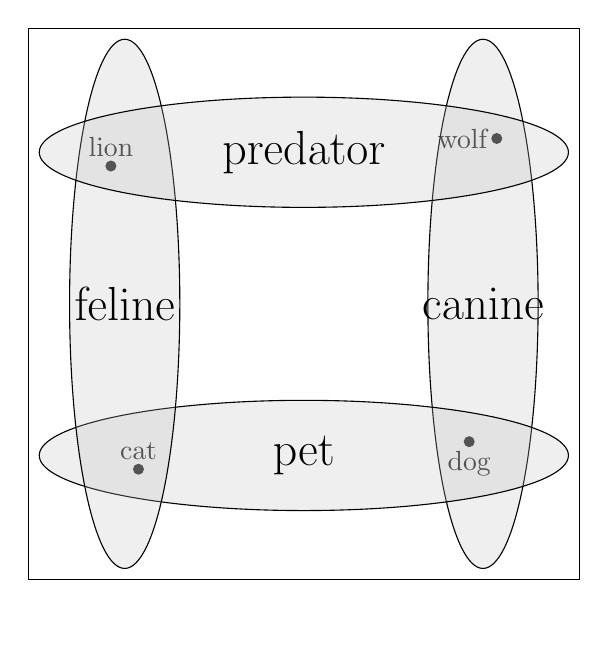
\begin{tikzpicture}[scale=0.07,baseline]
		\draw (0,0)--(-100,0)--(-100,-100)--(0,-100)--(0,0);
    	\draw (-15,-20) [left] node {wolf};
        \fill (-15,-20) circle[radius=1];
        \draw (-20,-75) [below] node {dog};
        \fill (-20,-75) circle[radius=1];
        \draw (-80,-80) [above] node {cat};
        \fill (-80,-80) circle[radius=1];
        \draw (-85,-25) [above] node {lion};
        \fill (-85,-25) circle[radius=1];
        \draw[fill=lightgray, fill opacity=0.25] (-17.5,-50) ellipse (10 and 48);
        \node at (-17.5,-50) {\LARGE canine};
        \draw[fill=lightgray, fill opacity=0.25] (-50,-77.5) ellipse (48 and 10);
        \node at (-50,-77.5) {\LARGE pet};
        \draw[fill=lightgray, fill opacity=0.25] (-82.5,-50) ellipse (10 and 48);
        \node at (-82.5,-50) {\LARGE feline};
        \draw[fill=lightgray, fill opacity=0.25] (-50,-22.5) ellipse (48 and 10);
        \node at (-50,-22.5) {\LARGE predator};
        \node at (-50,-102.5) [single arrow,draw,rotate=90,minimum height=40,minimum width=40,inner sep=15,opacity=0] {};
    \end{tikzpicture}
    \caption{a lexical space}
    \label{fig:bland}
    \end{subfigure}
    \begin{subfigure}[t]{0.5\textwidth}
    \centering
	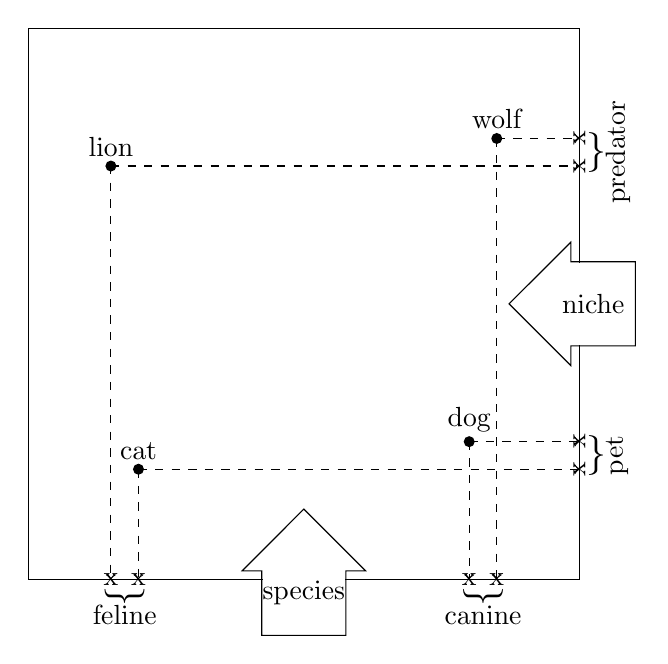
\begin{tikzpicture}[scale=0.07,baseline]
    	\draw (0,0)--(-100,0)--(-100,-100)--(-57.5,-100);
        \draw (-42.5,-100)--(0,-100)--(0,-57.5);
        \draw (0,-42.5)--(0,0);
    	\draw (-15,-20) [above] node {wolf};
        \fill (-15,-20) circle[radius=1];
        \draw[dashed,->] (-15,-20)--(-15,-100);
        \draw (-15,-100) node {x};
        \draw[dashed,->] (-15,-20)--(0,-20);
        \draw (0,-20) node [rotate=90] {x};
        
        \draw (-20,-75) [above] node {dog};
        \fill (-20,-75) circle[radius=1];
        \draw [dashed,->] (-20,-75)--(-20,-100);
        \draw (-20,-100) node {x};
        \draw [dashed,->] (-20,-75)--(0,-75);
        \draw (0,-75) node [rotate=90] {x};
        
        \draw (-80,-80) [above] node {cat};
        \fill (-80,-80) circle[radius=1];
        \draw [dashed,->] (-80,-80)--(-80,-100);
        \draw (-80,-100) node {x};
        \draw [dashed,->] (-80,-80)--(0,-80);
        \draw (0,-80) node [rotate=90] {x};
        
        \draw (-85,-25) [above] node {lion};
        \fill (-85,-25) circle[radius=1];
        \draw [dashed,->] (-85,-25)--(-85,-100);
        \draw (-85,-100) node {x};
        \draw [dashed,->] (-85,-25)--(0,-25);
        \draw (0,-25) node [rotate=90] {x};
        
        \node at (3,-22.5) [below,rotate=90] {predator};
        \node at (3,-22.5) {\Large\}};
		
        \node at (3,-77.5) [below,rotate=90] {pet};
        \node at (3,-77.5) {\Large\}};
		
        \node at (-17.5,-103) [below] {canine};
        \node at (-17.5,-103) [rotate=-90] {\Large\}};

        \node at (-82.5,-103) [below] {feline};
        \node at (-82.5,-103) [rotate=-90] {\Large\}};
        
        \node at (-50,-102.5) [single arrow,draw,rotate=90,minimum height=40,minimum width=40,inner sep=15] {};
        \node at (-50,-102.5) {species};
        \node at (2.5,-50) [single arrow,draw,rotate=180,,minimum height=40,minimum width=40,inner sep=15] {};
        \node at (2.5,-50) {niche};
    \end{tikzpicture}
    \caption{a contextual projection}
    \label{fig:reduce}
    \end{subfigure}
  \caption{In the two-dimensional space depicted in (a), the conceptual vagary of four words maps to overlapping, elongated and indeterminate spaces.  In (b), two different perspectives on the lexical space, represented by the arrows labelled \emph{niche} and \emph{species}, offer contextualised projections in one-dimensional clusters which remit conceptual clarity.}
\label{fig:perspective}
\end{figure}

Furthermore, the high dimensionality of vector space models of distributional semantics in particular should afford precisely these types of contextual viewpoints on potential relationships between words.  Rather than depending on \emph{a priori} disambiguation based on clustering or observations of context in the form of existing combinations of words, I propose that a technique for defining semantic subspaces \emph{in situ} will capture the momentary and situated way in which concepts come about in the course of a cognitive agent's entanglement with the world.  The way that relationships between words coalesce and then dissolve as we change our perspective on the space of this model is designed to reflect the way that concepts emerge dynamically in response to unfolding events in the world, and the ability to selectively specify the dimensional profile of a space of geometrically related semantic representations should enable just this kind of shifting of conceptual perspective.  The theoretical mechanisms for making choices about multi-dimensional perspectives in semantic spaces will be discussed in the next section.

\paragraph{A Note on \emph{Context}} The term \emph{context} has been used widely and varyingly by authors in both theoretical and computational linguistics, and with good reason, as various sense of the concept of context are clearly at play in any serious discussion of the interplay between language and cognition.  Statistically minded computational linguists in particular, of whom I would like to count myself as one, have often used \emph{context} to refer to the window of co-occurrence in which a word token is observed within a sample of text.  In his description of a co-occurrence statistic for measuring semantic similarity, \cite{Schutze1992b} introduced the term \emph{context space} to refer to a space of co-occurrence dimensions, a terminology subsequently adopted by \cite{BurgessEA1997} in relation to their HAL system.  This notion of proximity within a text as context has persevered in the natural language processing literature.

Theoretical linguists and cognitive scientists, on the other hand, have tended to treat \emph{context} as a much more general condition wrapped up with the entire perceptual, phenomenological aspect of existing as a cognitive agent in a complex world.  So for instance \citeauthor{Bateson1972} says that ``message material, or information, comes out of a context into a context,'' \cite[][p. 404]{Bateson1972}, meaning that there is an alignment between the inner context of an agent and the outer context of the world, while \citepos{Grice1975} notion of \emph{implicature} holds that meaning is somehow always determined in a context, with the exact nature of context remaining somewhat open-ended, and this nomenclature has been carried on by subsequent researchers interested in the idea that cognition, conceptualisation, and, correspondingly, language are always in some way specified by a situation in the world.  The idea is that context is probably something that exists in large part outside of language, and almost certainly outside the informationally restrictive confines of word co-occurrences within a sentence.

In this thesis, which seeks to address both those components of language measurable by an information processing system and the more general question of meaning as an environmentally situated phenomenon, I will endeavour to use the term \emph{context} strictly in reference to the latter notion of the situation in which concepts and semantics emerge in tandem.  With regard to words observed in proximity to one another, on the other hand, I will refer to \emph{co-occurrence}, and so additionally to a \emph{co-occurrence window} within which such observations are made and correspondingly a \emph{co-occurrence statistic} as a measure of the relative frequency of such observations.  Hopefully this terminological commit will serve to avoid confusion.

\section{Literal Dimensions of Co-Occurrence}
The model presented here is grounded within the paradigm of distributional semantics, which means that the conceptual geometries that it constructs are the product of observations of word co-occurrences in a large-scale corpus of textual data represented statistically.  Two procedurally distinct methodological regimens have emerged from the recent study of distributional semantics.  The first, and more established, approach involves tabulating word co-occurrence frequencies and then using some function over these to build up word-vector representations.  With roots in the frequentist analysis described by \cite{SaltonEA1975}, recent research has typically involved matrix factorisation techniques presented as either (or both) an optimisation method \citep{BullinariaEA2012} or a noise reducing mechanism \citep{KielaEA2014}.\footnote{\cite{BullinariaEA2012}, \cite{LapesaEA2013}, and \cite{KielaEA2014} have all reported that dimensional reduction techniques including SVD, random indexing, and top frequency feature selection generally do not improve results on word similarity and composition tests, with some notable parameter specific exceptions.}  A more recent approach, which has received a great deal of attention with the increasing availability of large-scale data and the corresponding advent of complex neural network architectures, involves using machine learning techniques to iteratively learn word-vector representations in an online, stepwise traversal of a corpus \citep{BengioEA2003,CollobertEA2008,KalchbrennerEA2014}.  \cite{BaroniEA2014} have described the former as \emph{counting} and the latter as \emph{predicting}, but it must be noted that both methods are very much grounded in observations about the co-occurrence characteristics of vocabulary words across large bodies of text.

Another important similarity between these two approaches is that they each in their own way move towards a representation of relationships between word-vectors which is to some extent optimally informative, and, by the same token, abstract.  In the instance of neural network approaches, this is clearly the case due to the fundamental nature of the technique: the dimensions of this variety of model exist as basically arbitrary handles for gradually adjusting the relative positions of vectors, slightly altering every dimension of each vector each time the corresponding word is observed in the corpus.  And, as far as models based on explicit co-occurrence counts are concerned, the favoured technique tends to involve starting with a large, sparse space of raw co-occurrence statistics (frequencies, or, more typically, an information theoretic type metric) and then factorising this matrix using a linear algebraic technique such as singular value decomposition.  The result, in either case, is a space of vectors which exists just for the sake of placing words in a relationship where distance corresponds to a semantic property, consisting of dimensions which can only be interpreted in terms of the way that they allow the model to relate words, not in terms of their relationship to the underlying data.  In fact, \cite{LevyEA2014b} have argued that recently developed neural network approaches just exactly recapitulate the process of matrix factorisation, and that a careful tuning of hyperparameters will generate commensurable results from either type of model.

A key feature of the methodology proposed in this thesis is that it maintains a base space of highly sparse co-occurrence statistics, which, despite their anchoring in the relatively abstract realm of word positions in a digitised corpus, I will describe as \emph{literal} in the sense that they can be interpreted as corresponding to actual relationships between word tokens in the world.  As mentioned in the previous section, a fundamental objective of this methodology is to afford an abundance of potential perspectives on co-occurrence data.  This objective is accomplished by providing a model with a corresponding proliferation of dimensions from which to make projections by way of context specific selections of subsets of dimensions.  Furthermore, by maintaining the literal connection between the dimensions and the underlying data, the methodology likewise sustains a mechanism for selecting the dimensions in a way that is fundamentally interpretable, in that we can predict something about the geometric contribution of a given dimension to a subspace based on the types of words which tend to co-occur with that dimension.  The co-occurrence profiles of the dimensions themselves will become an important criterion for dimensional selection, and having a very large set of such profiles to analyse will give a semantic model great scope in its capacity for adopting situational perspectives on the relationships between words.

%I don't wish to claim that there is scope for completely or even mainly recapitulating a nuanced conceptual model from the data available in a purely textual environment; to do so would be to move towards claims that intentionality can emerge from rule-based operations on symbols, and the problems with this have been explored by \citepos{Searle1980} Chinese room argument and a subsequent generation of philosophers \citep{PrestonEA2002}.  But I would like to suggest that by building a base model that maintains the accessibility of unreduced co-occurrence information, we likewise maintain the ability to manipulate this base model extemporaneously, in reaction to the ongoing emergence of new contextual information.  The idea is that such a base model would essentially represent the superset of all possible dimensions available for \emph{ad hoc} selection in the course of a 

So the proper framework for describing the model to be examined in this thesis is not so much a single space of word-vectors as a Grassmannian lattice consisting of the power set of all possible combinations of the dimensions characterising the base space.  At the top of this lattice -- the \emph{join} -- sits a single $d$-dimensional space consisting of every available one of the $d$ co-occurrence terms observed throughout the underlying corpus.  At the bottom of the lattice -- the \emph{meet} -- sit $d$ different one-dimensional spaces, each space corresponding to a single co-occurrence term.  If the meet is considered layer-$1$ of the lattice, and the join is considered layer-$d$, then any given interstitial layer-$j$ consists of every possible combination of $j$ dimensions of co-occurrence statistics.  A diagram of a very simple example of one such model is presented in Figure~\ref{fig:lattice}, illustrating the possible subspaces projected from a vastly simplified model consisting of just three co-occurrence dimensions (these particular spaces will be explored in the next section, providing the basis for the interpretable geometries illustrated in Figure~\ref{fig:instruments}).

\begin{figure}
\centering
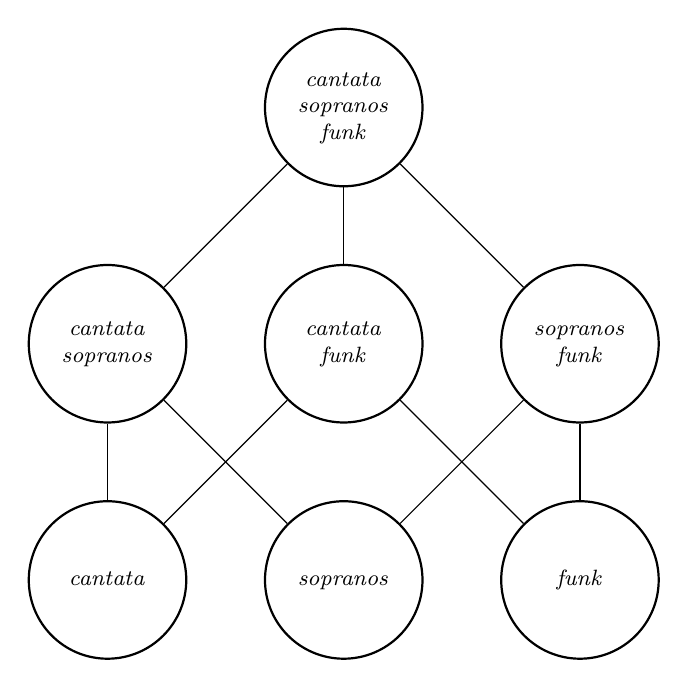
\begin{tikzpicture}[node distance=3cm,every node/.style={draw=black,thick,circle,inner sep=0pt}]
  \footnotesize
  \node[minimum size=2cm](join) {\begin{tabular}{c}
    \emph{cantata} \\
    \emph{sopranos} \\
    \emph{funk}
  \end{tabular}};
  \node[minimum size=2cm](two2) [below of=join] {\begin{tabular}{c}
    \emph{cantata} \\
    \emph{funk}
  \end{tabular}};
  \node[minimum size=2cm](two1) [left of=two2] {\begin{tabular}{c}
    \emph{cantata} \\
    \emph{sopranos}
  \end{tabular}};
    \node[minimum size=2cm](two3) [right of=two2] {\begin{tabular}{c}
    \emph{sopranos} \\
    \emph{funk}
  \end{tabular}};
  \node[minimum size=2cm](one2) [below of=two2] {\begin{tabular}{c}
    \emph{sopranos}
  \end{tabular}};
  \node[minimum size=2cm](one1) [left of=one2] {\begin{tabular}{c}
    \emph{cantata}
  \end{tabular}};
  \node[minimum size=2cm](one3) [right of=one2] {\begin{tabular}{c}
    \emph{funk}
  \end{tabular}};
  \draw (two1)--(join);
  \draw (two2)--(join);
  \draw (two3)--(join);
  \draw (one1)--(two1);
  \draw (one1)--(two2);
  \draw (one2)--(two1);
  \draw (one2)--(two3);
  \draw (one3)--(two2);
  \draw (one3)--(two3);
\end{tikzpicture}
\caption{A lattice of three dimensions, including the two-dimensional subspaces which are used for analysing the conceptual geometry of a small set of word-vectors in Figure~\ref{fig:instruments}}
\label{fig:lattice}
\end{figure}

An important distinction must be drawn, however, between the representation of my model as a lattice and the use of manifolds as an inferential mechanism.  Formal concept analysis in particular has made a productive discipline out of applying lattice type structures to conceptual modelling, using the semi-hierarchical properties of lattices to capture logical relationships of entailment \citep{Wille1982}.  That body of work takes as given that concepts are ``the basic units of thought formed in dynamic processes within social and cultural environments,'' \citep[][p. 2]{Wille2005}.  \cite{Widdows2004} offers a broad overview of how this approach might be pursued through corpus linguistic techniques, while \cite{GeffetEA2005} and, more recently, \cite{KartsaklisEA2016} have proposed statistical techniques using \emph{feature inclusion} metrics to assess the potential entailment relationships between candidate words and corresponding concepts.  The assumption inherent in this interesting work is that words are in some sense supervenient upon the concepts they denote, and that the statistical features of a language will by and large recapitulate the conceptual structure upon which it sits.

As \cite{Rimell2014} has pointed out, however, it is problematic to assume that a spectrum of co-occurrence alone can indicate relationships of hyponymy and hypernymy.  It stands to reason, for instance, that a word with a taxonomically specific denotation such as \emph{bulldog} should probably have a co-occurrence profile including words omitted from the corresponding profile of a word like \emph{lifeform}, which has an ostensibly more general extension---even excluding some of the ambiguity inherent in \emph{bulldog}, it seems reasonable to talk about a \emph{pet bulldog} but less so to talk about a \emph{pet lifeform}, for instance.  Rimell has proposed a measure of change in \emph{topic coherence} as word-vectors are combined algebraically in order to detect entailment relationships.  This measuring is achieved specifically through a process of dimension-by-dimensions comparison between potentially related word-vectors, in particular the \emph{vector negation} method described by \cite{Widdows2003}, combined with topic modelling techniques to analyse the coherence of features distilled by the selectional process.

The methodology proposed in this thesis adheres to the same principle of fine-grained cross-dimensional analysis described by Rimell.  In addition to the practical issues raised by Rimell, my approach is also designed to remain pointedly uncommitted to any claim that concepts are atomic or elementary to thought, or that language and concepts are involved in any kind of strictly hierarchical interrelationship.  Instead, my models operate through an analytical traversal of lattices of subspaces in search of combinations of dimensions that capture conceptually \emph{salient} profiles of co-occurrence features.  If a consequence of this stance is that a model built from this methodology can't be understood in terms of nested, ordered relationships, though, then the question of how conceptual relationships do emerge situationally from the methodology remains.  The next section of this theoretical overview will examine how the actual geometry of a projected subspace itself is expected to do this conceptual work.

\section{Interpretable Geometry}
It is important at this point to distinguish between two different modes of interpretability at play within the operation of the methodology I'm proposing.  On the one hand, we have the process for selecting subspaces described above: this process requires a model composed of tractable dimensions of statistics that can be interpreted based on expectations generated from an analysis of some sort of contextually relevant information.  Some specific mechanisms for this process will be discussed in the next chapter.  Then on the other hand, once this selectional process has taken place, we find ourselves with a subset of dimensions defining a specific subspace.  My claim is that, given the correct selectional criteria for performing this projection -- this traversal of our lattice of vector spaces -- we should be able to generate a subspace in which the projected word-vectors will be interpretable in terms of the actual geometric features of this subspace.

The idea of exploiting the geometry of a transformed space of word statistics is not new.  Indeed, seminal work on latent semantic analysis was motivated by precisely the insight that a singular value decomposition of a high-dimensional, sparse matrix of statistical data about word co-occurrences would result in a dense lower dimensional matrix in which dimensions characterise \emph{latent semantics} rather than literal word co-occurrences \citep{DeerwesterEA1990}.  Thus the linear algebraic methodology of generating a lower dimensional matrix of optimally informative dimensions arguably transforms a space of specific co-occurrence tendencies into a space of more general conceptual relationships.  In fact, \citeauthor{LandauerEA1997} have subsequently argued that the dimensional reduction by way of factorisation itself might directly mirror cognitive conditioning, modelling the way that the mind can ``correctly infer indirect similarity relations only implicit in the temporal correlations of experience,'' \citep[][p. 212]{LandauerEA1997}.

Of course the dimensions of a factorised matrix are still not interpretable in themselves.  They are, rather, an optimal abstraction of the underlying data, in which each dimension is maximally informative -- and, accordingly, orthogonal -- in comparison to the other dimensions.  What we desire in a model, however, is a mechanism for actually interpreting directions and regions within a subspace projected by the model.  This objective is motivated by \citepos{Gardenfors2000} insight into the inferential power of \emph{conceptual spaces}: by building spaces in which the dimensions themselves correspond to \emph{properties}, G\"{a}rdenfors has illustrated how features of points and regions within these spaces such as convexity and betweeness can be interpreted as corresponding to conceptual membership and can accordingly be used to reason about relationships between concepts.  In more recent work, motivated by psycholinguistic insight into the significance of the \emph{intersubjectivity} by which language facilitates the mutual ascription of cognitive content between interlocutors, \cite{Gardenfors2014} has proposed that semantics are derived from a communicative alignment of conceptual spaces.

A classic example of a G\"{a}rdenforsian conceptual space is the space of colours, which can be defined in terms of, for instance, hue, brightness, lightness, and colourfulness: any colour percept can be specified as a point corresponding to coordinates along each of these dimensions.  Moreover, regions within the space of colours can be defined geometrically: the concept \textsc{red} will correspond to a convex region within the space, and any point lying between two points known to be labelled \emph{red} will likewise be considered \textsc{red}.  \cite{Jager2010} has devised an experiment mapping linguistic descriptions to conceptual regions precisely within the domain of colours.  Taking a large set of multi-lingual data regarding colour naming conventions and treating each of 330 different colours as an initially independent dimension, J\"{a}ger demonstrated how an extrapolation of optimally informational dimensions via a principle component analysis revealed clusterings of colour names into convex regions.\footnote{The cross-cultural universality of colour naming conventions presented by \cite{KayEA1999}, which J\"{a}ger takes as a basis for his research, is controversial to say the least -- see \cite{Levinson2001} for an alternative point of view -- but J\"{a}ger's work remains a good example of a computational technique for extrapolating conceptual spaces from quantitative linguistic data.}

Similarly motivated by G\"{a}rdenfors's model of conceptual spaces, \cite{DerracEA2015} have built vectors of domain specific documents, associating word frequencies within documents with document labels.  A multi-dimensional scaling procedure is then used to project these document-vectors into a Euclidean space in which the authors predict that properties such as \emph{parallelness} and \emph{betweeness} will correspond to conceptual relationships between documents.  The authors demonstrate that geometry in their projected spaces does indeed afford conceptual interpretation: the vector they construct from large scale textual data for the word \emph{bog} is found to be more or less between the vectors for \emph{heath} and \emph{wetland}, for instance, and the vector for the film \emph{Jurassic Park} lies in directions associated with \textsc{dinosaurs} and \textsc{special effects}.  This work is particularly notable in that \citeauthor{DerracEA2015} appreciate the significance of projecting spaces which are interpretable in terms of Euclidean distances rather than simply the cosine similarity of vectors extending from the origin of a space: Euclidean metrics provide a platform for more nuanced considerations of the relationships between points.

The type of space exemplified by the research of J\"{a}ger and \citeauthor{DerracEA2015} is moving towards being a conceptual space in the way that its geometry offers itself up to semantic interpretation, but importantly these remain static spaces comprised of abstract dimensions, albeit dimensions generated in order to optimise the interpretability of the spaces they delineate.  The objective of my model is to emulate the geometric interpretability of these other spaces in an extemporaneous, contextually dynamic way.  To illustrate this point, consider the two spaces illustrated in Figure~\ref{fig:instruments} (taken from real co-occurrence data, as described in the next chapter, and based on the lattice of subspaces illustrated in Figure~\ref{fig:lattice}).  Here co-occurrence statistics are used to define three different dimensions, from which two different two-dimensional subspaces are selected with word-vectors plotted into each subspace.  In each subspace, a particular conceptual geometry emerges, oblique to the axes of each subspace but nonetheless indicating distinct conceptual regions in which words align themselves in an interpretable way.

\begin{figure}[t]
	\begin{subfigure}[t]{0.5\textwidth}
    \centering
	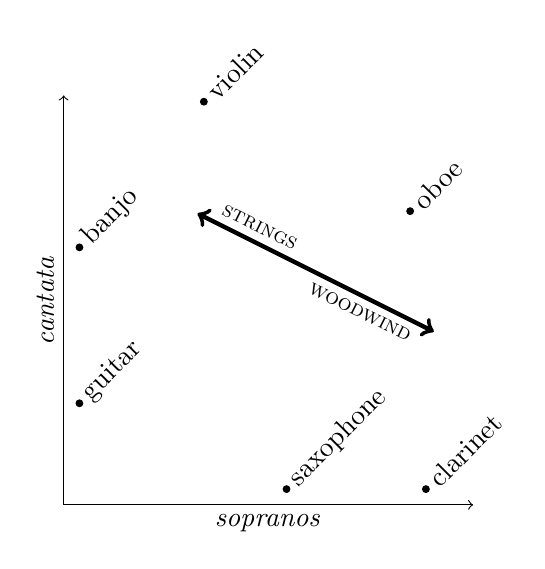
\begin{tikzpicture}[scale=1,baseline]
		\draw [->] (-0.2,-0.2)--(5,-0.2);
		\draw [->] (-0.2,-0.2)--(-0.2,5);
		\node at (2.4,-0.2) [below] {\emph{sopranos}};
		\node at (-0.2,2.4) [above,rotate=90] {\emph{cantata}};
		\draw [<->,ultra thick] (1.5,3.5)--(4.5,2);
		\node at (2.2,3.15) [above,rotate=-26.57] {\footnotesize \textsc{strings}};
		\node at (3.65,2.425) [below,rotate=-26.57] {\footnotesize \textsc{woodwind}};
		\node at (0.0,1.09) [right,rotate=45] {guitar};
		\fill (0.0,1.09) circle[radius=0.05];
		\node at (0.0,3.07) [right,rotate=45] {banjo};
		\fill (0.0,3.07) circle[radius=0.05];
		\node at (1.58,4.92) [right,rotate=45] {violin};
		\fill (1.58,4.92) circle[radius=0.05];
		\node at (2.63,0.0) [right,rotate=45] {saxophone};
		\fill (2.63,0.0) circle[radius=0.05];
		\node at (4.40,0.0) [right,rotate=45] {clarinet};
		\fill (4.40,0.0) circle[radius=0.05];
		\node at (4.20,3.53) [right,rotate=45] {oboe};
		\fill (4.20,3.53) circle[radius=0.05];
    \end{tikzpicture}
    \caption{\textsc{strings} vs \textsc{woodwind}}
    \label{fig:svsw}
    \end{subfigure}
    \begin{subfigure}[t]{0.5\textwidth}
    \centering
	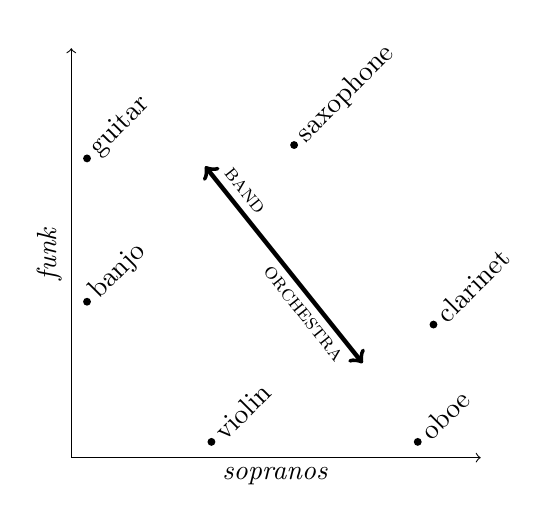
\begin{tikzpicture}[scale=1,baseline]
		\draw [->] (-0.2,-0.2)--(5,-0.2);
		\draw [->] (-0.2,-0.2)--(-0.2,5);
		\node at (2.4,-0.2) [below] {\emph{sopranos}};
		\node at (-0.2,2.4) [above,rotate=90] {\emph{funk}};
		\draw [<->,ultra thick] (1.5,3.5)--(3.5,1);
		\node at (1.85,3.0625) [above,rotate=-51.35] {\footnotesize \textsc{band}};
		\node at (2.9,1.75) [below,rotate=-51.35] {\footnotesize \textsc{orchestra}};
		\node at (0.0,3.60) [right,rotate=45] {guitar};
		\fill (0.0,3.60) circle[radius=0.05];
		\node at (0.0,1.78) [right,rotate=45] {banjo};
		\fill (0.0,1.78) circle[radius=0.05];
		\node at (1.58,0.0) [right,rotate=45] {violin};
		\fill (1.58,0.0) circle[radius=0.05];
		\node at (2.63,3.77) [right,rotate=45] {saxophone};
		\fill (2.63,3.77) circle[radius=0.05];
		\node at (4.40,1.49) [right,rotate=45] {clarinet};
		\fill (4.40,1.49) circle[radius=0.05];
		\node at (4.20,0.0) [right,rotate=45] {oboe};
		\fill (4.20,0.0) circle[radius=0.05];
    \end{tikzpicture}
    \caption{\textsc{band} vs \textsc{orchestra}}
    \label{fig:bvso}
    \end{subfigure}
  \caption{Based on real co-occurrence data, swapping one dimension in a two-dimensional subspace reveals two different conceptual geometries.}
  \label{fig:instruments}
\end{figure}

The first thing to note about these spaces is the way that swapping a single dimension in a two dimensional subspace can have a significant impact on the conceptual affordances of the subspace's geometry.  Realigning the relationships between terms along a single axis leads to a complete shift in the groupings of terms, and, correspondingly, to the interpretation of regions and directions.  If these are conceptually sound subspaces, then we might expect word-vectors found within the area of the triangle described by the points labelled \emph{guitar}, \emph{banjo}, and \emph{violin} in Figure~\ref{fig:svsw} to be the names of other string instruments, or other conceptually relevant terms.  This is possibly asking too much of a subspace consisting of data regarding co-occurrences with just two terms across a large scale corpus, but as we scale up the dimensionality of the space -- as we ascend the lattice of subspaces of a fully realised model -- we can expect proper conceptual spaces to begin to coalesce.

The next thing to note is that the dimensions themselves are not especially interpretable.  While these dimensional profiles are explicable -- and indeed the ability to trace these statistics back to the corpus might turn out to be a desirable property for some applications -- the dimensions themselves do not conform to \citepos{Gardenfors2000} notion of dimensions as representing the properties that compose a concept.  It might be surprising, for instance, that the word \emph{cantata} has a higher propensity for co-occurrence with the word \emph{banjo} than with the word \emph{clarinet}, given that cantatas have traditionally included parts for the latter but not the former.  An examination of the underlying data, extracted, as described in the next chapter, from English language Wikipedia, reveals that the term \emph{cantata} has been adopted, perhaps somewhat figuratively, by some bluegrass musicians, and so co-occurrences with \emph{banjo} are indeed observed.

Rather than consider such usage as anomalous or attempt some sort of \emph{a priori} word sense disambiguation, I propose to embrace the haphazardness of language and use it as a tool for projecting conceptually productive geometries.  In fact it would be surprising if it turned out that in anything other than the most specialised cases we could simply pick dimensions based on their labels and then expect co-occurrence statistics to play out in a conceptually coherent way, as this would contradict the Relevance Theoretic thesis that language in use is always significantly underspecified.  With this in mind, I suggest that we consider some set of dimensions, delineating a subspace and the corresponding geometry of word-vectors, to map precisely to a given context, and to effectively serve as the connective structure between language and conceptualisation.  Under this regimen, the dimensions themselves become the constitutive substance of a context, but they do not compositionally define any context in which they participate; rather, the contextualisation is an emergent property of the combination of dimensions underwriting it, corresponding to \emph{a way of speaking} about things.

The spaces illustrated in Figure~\ref{fig:instruments} are the product of a survey of a lattice consisting of combinations of just three dimensions, and as such the conceptual affordances of this toy model are highly limited.  As we add dimensionality to the model, however -- as we observe more terms co-occurring with our vocabulary of word-vectors -- we can expect an exponential growth in the combinatory possibilities of subspace construction.  With enough dimensions from which to choose, and with an appreciable degree of variance between the profiles of each dimensions, there should be scope for projecting more or less any constellation of word-vectors we desire.  The next question, then, is how to go about actually extracting a high dimensional base model of co-occurrence statistics from a large scale textual corpus and then explore the conceptual possibilities of this base space's inherent subspaces.  The next chapter will answer this question.

%\section{A Computational Process}
%In this final section of this chapter, a technical implementation of the model described throughout the preceding three sections will be explained in detail.

%\subsection{A Large Scale Textual Corpus}
%The first step in a corpus based approach to natural language processing is the selection of the data which will provide the basis for our model.  I've picked the English language portion of Wikipedia as my data source, a choice which is in accordance with a good deal of work done in the field.  Some authors 

%In the case of the model used throughout this thesis, the November 2014 dump of English language Wikipedia has been used.\footnote{Accessible at XXX}  A data cleaning process has been implemented, the first step of which is the chunking of the corpus into individual sentences.  Next parenthetical phrases are removed from each sentence, as these can potentially skew co-occurrence data, and all other punctuation is subsequently removed.  All characters are converted into lowercase to avoid words capitalised at the beginning of sentences, quotations, and other places from being considered as unique types.  Finally, the articles \emph{a}, \emph{an}, and \emph{the} are removed as they can distort co-occurrence windows (consider, for instance, how these terms affect the proximity of the other words in the phrase ``a mouse, an owl, and a dog sat on the moon'').  The cleaned corpus contains about

%-WORD, SENTENCE COUNTS

%As is generally the case with data cleaning, these measures are prone to error: for instance, due to the removal of punctuation, the contraction \emph{we're} will be considered identical to the word \emph{were}.  One of the strengths of the subspace projection technique that my model uses is its resilience to noise.  So, for instance, misspellings will be categorised as highly anomalous co-occurrence dimensions and are therefore unlikely to be contextually selected -- or, if they are regularly encountered enough to be contextually significant, there may well be useful information in the co-occurrence profile of such mistakes -- and essentially ubiquitous words are unlikely to provide context specific information, so the ambiguity between \emph{we're} and \emph{were} is unlikely to be drawn into any of the subspaces actually projected by the model.

%From the cleaned corpus, the model's vocabulary is defined as the top 200,000 most frequently occurring word types.  This cut-off point is very close to the point where the total number of word tokens included -- that is, occurrences of any word of any type -- included by selecting all instances of all vocabulary words equals the total number of word types -- that is, unique word forms -- excluded.  Given the Zipfian distribution of word frequencies as observed throughout the corpus, this means that more than 95\% of the co-occurrence data available from the corpus will be taken into account by the model, while the number of word-vectors used to express this data represents less than 5\% of the potential vocabulary---a fairly efficient way of extrapolating statistics from the corpus.

%- human vocabulary size

%\subsection{Mutual Information of Word Co-Occurrences}
%The critical event in the 

%Here, following the example of almost all distributional semantic work, co-occurrence between a word $w$ and another word $c$ will be considered in terms of the number of other words between $w$ and $c$.  In the case of my model, again in accord with the a great deal of work within the field, a statistic for word $w$ in terms of its co-occurrence with $c$ will be derived from the consideration of all the times that $c$ is observed within $k$ words of $w$, where $k$ is one of the primary model parameters that will be considered in the experiments reported in later chapters of this thesis.  Based on these co-occurrence events, a matrix $M$ is defined, where rows consist of word-vectors, one for each of the 200,000 words in the vocabulary, and columns correspond to terms with which these vocabulary words co-occur.  These column-wise co-occurrence dimensions include the words in the vocabulary, including the possible co-occurrence of a word with itself (``a \emph{rose} is a \emph{rose} is a \emph{rose}'', for instance) as well as many, many words that are not in the vocabulary, to the extent that every word type in the corpus is considered as a dimension of co-occurrence.

%In this last respect, my model diverges from the typical approach, which usually seeks to limit not only the vocabulary but also the dimensionality of the underlying co-occurrence matrix.  This has typically involved a curtailing of the number of co-occurrence terms at both ends of the frequency spectrum, based on the assumption that both high frequency so-called function words (the prepositions, conjunctions, and so forth) and low frequency terms such as obscure proper names will muddy a model with either general flattening or highly topical skewing.  In the case of my model, however, these problems are irrelevant, as dimensions will be selected on a case-by-case, context specific basis, and there is no good reason to discard information which may in some possibly unforeseen circumstance prove relevant.  The result is a 200,00 by $\approx$ 7.5 million matrix $M$ where a scalar corresponding to co-occurrences between $w$ and $c$ is defined in terms of this equation:

%\begin{equation}\label{eq:MI}
%M_{w,c} = \log_2 \left(\frac{n_{w,c} \times W}{n_w \times \left(n_c + a\right)} + 1\right)
%\end{equation}

%Here $n_{w,c}$ represents the total number of times that that $c$ is observed as co-occurring in a sentence within $k$ words on either side of $w$, $n_w$ is the independent frequency of occurrences of $w$, and $c$ is likewise the overall frequency of $c$ being observed as a co-occurrence term throughout the corpus.  $W$ is the overall occurrence of all words throughout the corpus---and it should be noted that, excluding the term $a$, the ratio in Equation~\ref{eq:MI} is equivalent to the joint probability of $w$ and $c$ co-occurring.  The application of a logarithm to this ratio, again a common practice, is in the spirit of \citepos{Shannon} information theory, and is 

%The term $a$ is a skewing constant used to prevent highly specific co-occurrences from dominating the analysis of a word's profile, set for the purposes of the work reported here at 10,000.\footnote{Anecdotally, the first combination of input words analysed during an early stage of the development of this model that didn't use a smoothing constant was the phrase ``musical creativity'', and the very first dimension indicated by the analysis was labelled \emph{gwiggins}---my primary supervisor's email handle.  Prof. Wiggins's deep connection with music and creativity meant that every instance of \emph{gwiggins} occurring throughout Wikipedia was in the vicinity of both \emph{musical} and \emph{creativity}, and so the dimension was indicated by the combination of these terms, which makes sense, but it was still a bit eerie to have such a personally relevant result generated by a model based on such general data.}

%Finally, the entire ratio is skewed by 1 so that all values returned by the logarithm will be greater than 0, with a value of zero therefore indicating that two words have never been observed to co-occur with one another.  This is again a departure from standard practice, where, in word counting models, a \emph{pointwise mutual information} mechanism involving not skewing the ratio and instead treating any ratio of frequencies less than 1 -- that is, any co-occurrence that is observed less than often than balance of the mean values for all occurrences of $w$ and all co-occurrences with $c$ -- as being equivalent to 0, or no co-occurrence at all.  The motivation for this more typical technique is again to avoid incorporating unnecessary and potentially confounding information into a model, but, again, in the case of my model, the dimensional selection process will tend to ignore such information, and at the same time, as will be seen, data regarding relatively unlikely co-occurrences can sometimes also be quite informative.  In support of my technique, it is worth mentioning that the vast majority of potential co-occurrences will never be observed, and, at the same time, a comprehensive language model should maintain at least the possibility of any co-occurrence

%\cite{Brown}

%so there seems to be wisdom in the idea of not throwing away information about even relatively unlikely linguistic events.

%\subsection{Dimensional Selection Techniques}
%Having established a base model of co-occurrence statistics, the 

%\begin{equation}\label{eq:oldNorm}
%w^j_i = \frac{w^j_i}{\sqrt{\sum_{k=1}^{b} \left(w^k_i\right)^2}}
%\end{equation}

%\begin{equation}\label{eq:Norm}
%w^j_i = \frac{w^j_i}{\sum_{k=1}^{b} abs\left(w^k_i\right)}
%\end{equation}

%\begin{equation}\label{eq:Arg}
%\mu_c =  \frac{1}{n} \sum_{w=1}^{n}N_{w,c}
%\end{equation}

%\begin{equation}\label{eq:Trans}
%M_{w,c} \Rightarrow S_{w,c'}
%\end{equation}
%\subsection{Extracting Semantics from Geometric Features}

\chapter{A Computational Implementation of Context Sensitive Distributional Semantics} \label{chap:method}
In the previous chapter, I laid the theoretical groundwork for a distributional semantic methodology for dynamically establishing perspectives on statistical data about language use.  In this chapter, I'll describe the technical details for building a computational implementation of such a methodology.  The objective of this implementation is to establish a rigorous procedure for generating subspaces of word vectors, based on observations of word co-occurrences in an underlying corpus, the geometries of which are semantically productive in particular contexts.  This will involve three steps:

\begin{enumerate}
\item The selection, processing, and analysis of a large scale textual corpus in order to create a high dimensional base space of co-occurrence statistics;
\item The development of techniques for selecting lower dimensional subspaces based on some sort of contextualising input;
\item The exploration of the geometry of the projected subspaces in search of semantic correlates.
\end{enumerate}

The following three sections will pursue each of these aspects of a technical implementation in turn.  The end result is effectively a mapping from text as raw data to geometry as semiotic generator.  A fourth section will describe an alternative, general interpretation of the statistical data which underwrites my models and additionally offer a brief overview of another distributional semantic methodology, all to be used as a point of comparison in the empirical results which will be discussed in subsequent chapters.

\section{Establishing and Analysing a Large Scale Textual Corpus}
The first step in a corpus based approach to natural language processing is the selection of the data which will provide the basis for our model.  I've picked the English language portion of Wikipedia as my data source, a choice which is in accordance with a good deal of work done in the field.  For instance, \cite{GabrilovichEA2007} and \cite{CollobertEA2008}, to name just a couple, use Wikipedia as their base data for training distributional semantic models designed to perform tasks similar to the ones explored in subsequent chapters, while \cite{Baroni2014}, \cite{PenningtonEA2014}, and \cite{GutierrezEA2016} use amalgamated corpora that include Wikipedia as a major component.  Wikipedia provides a very large sample of highly regular language, meaning that we can expect a certain syntactic and semantic consistency as well as language which, if not always overtly literal, is likewise not typically abstruse or periphrasitc.  This should supply a source of linguistic data in which, to revisit the central dogma of the distributional hypothesis, words which occur in a specific syntactic and lexical setting can be expected to be semantically similar.

In the case of my implementations, the November 2014 dump of English language Wikipedia has been used.\footnote{Relatively recent Wikipedia dumps are available at \url{https://dumps.wikimedia.org/}.}  A data cleaning process has been implemented, the first step of which is the chunking of the corpus into individual sentences.  Next parenthetical phrases are removed from each sentence, as these can potentially skew co-occurrence data, and all other punctuation is subsequently removed.  All characters are converted into lowercase to avoid words capitalised at the beginning of sentences, quotations, and other places being considered as unique types.  Finally, the articles \emph{a}, \emph{an}, and \emph{the} are removed as they can distort co-occurrence distance counts.  The cleaned corpus contains nearly 1.1 billion word tokens, consisting of almost 7.5 million unique word types.  The distribution of these types is predictably Zipfian: over 10 million occurrences of the top nine word types are observed, while the least frequent 4.27 million words -- more than half of all types -- only occur once.  The top end of this distribution is populated by conjunctions, prepositions, and pronouns, while the bottom end is characterised by obscure place names, one-off abbreviations, unicode representing non-Latin alphabet spellings, and a good many spelling errors.

As is generally the case with data cleaning, these measures are prone to error: for instance, due to the removal of punctuation, the contraction \emph{we're} will be considered identical to the word \emph{were}.  One of the strengths of the subspace projection technique that my methodology uses is its resilience to noise.  So, for instance, misspellings will be categorised as highly anomalous co-occurrence dimensions and are therefore unlikely to be contextually selected -- or, if they are regularly encountered enough to be contextually significant, there may well be useful information in the co-occurrence profile of such mistakes -- and, at the other end of the spectrum, essentially ubiquitous words are unlikely to provide context specific information, so the ambiguity between \emph{we're} and \emph{were} is unlikely to be drawn into any of the subspaces actually projected by the model.

From the cleaned corpus, a model's vocabulary is defined as the top 200,000 most frequently occurring word types.  This cut-off point is very close to the point where the total number of word tokens included -- that is, occurrences of any word of any type -- by selecting all instances of all vocabulary words equals the total number of word types -- that is, unique word forms -- excluded.  Given the Zipfian distribution of word frequencies as observed throughout the corpus, this means that more than 95\% of the co-occurrence data available from the corpus will be taken into account by the model, while the number of word-vectors used to express this data represents less than 5\% of the potential vocabulary---a fairly efficient way of extrapolating statistics from the corpus.  The selection of this as a cut-off point means that the least frequent words in the vocabulary occur 83 times throughout the corpus.

Having processed the corpus and established the target vocabulary, the next step of this methodology is to build up a based space of co-occurrence statistics.  Here, following the example of the majority distributional semantic work, co-occurrence between a word $w$ and another word $c$ will be considered in terms of the number of other words between $w$ and $c$.  In the case of my methodology, and again in accord with the a great deal of work within the field, a statistic for word $w$ in terms of its co-occurrence with $c$ will be derived from the consideration of all the times that $c$ is observed within $k$ words of $w$, where $k$ is one of the primary model parameters that will be considered in the experiments reported in later chapters of this thesis.  Based on these co-occurrence events, a matrix $M$ is defined, where rows consist of word-vectors, one for each of the 200,000 words in the vocabulary, and columns correspond to terms with which these vocabulary words co-occur.  These column-wise co-occurrence dimensions include the words in the vocabulary as well as many, many words that are not in the vocabulary, to the extent that every word type in the corpus is considered as a candidate for co-occurrence.  A \emph{pointwise mutual information} metric gauging the unexpectedness associated with the co-occurrence of two words is calculated in terms of this equation:

\begin{equation}\label{eq:MI}
M_{w,c} = \log_2 \left(\frac{f_{w,c} \times W}{f_w \times \left(f_c + a\right)} + 1\right)
\end{equation}

Here $f_{w,c}$ represents the total number of times that $c$ is observed as co-occurring in a sentence within $k$ words on either side of $w$, $f_w$ is the independent frequency of occurrences of $w$, and $f_c$ is likewise the overall frequency of $c$ being observed as a co-occurrence term throughout the corpus.  $W$ is the overall occurrence of all words throughout the corpus--and it should be noted that, excluding the term $a$, the ratio in Equation~\ref{eq:MI} is equivalent to the joint probability of $w$ and $c$ co-occurring.  The term $a$ is a skewing constant used to prevent highly specific co-occurrences from dominating the analysis of a word's profile, set for the purposes of the work reported here at 10,000.\footnote{Anecdotally, the first combination of input words analysed during an early stage of the development of this model that didn't use a smoothing constant was the phrase ``musical creativity'', and the very first dimension indicated by the analysis was labelled \emph{gwiggins}---the email handle of one of my supervisors.  Prof. Wiggins's deep connection with music and creativity meant that every instance of \emph{gwiggins} occurring throughout Wikipedia was in the vicinity of both \emph{musical} and \emph{creativity}, and so the dimension was indicated by the combination of these terms, which makes sense, but it was still a bit eerie to have such a personally relevant result generated by a model based on such general data.}  Finally, the entire ratio is skewed by 1 so that all values returned by the logarithm will be greater than 0, with a value of zero therefore indicating that two words have never been observed to co-occur with one another.

This last step of incrementing the ratio of frequencies in order to avoid values tending towards negative infinity in the case of very unlikely co-occurrences is again a departure from standard practice, where, in word counting models, a \emph{positive pointwise mutual information} mechanism involving not skewing the ratio and instead treating any ratio of frequencies less than 1 -- that is, any co-occurrence that is observed less often than the balance of the mean values for all occurrences of $w$ and all co-occurrences with $c$ -- as being equivalent to zero, or no co-occurrence at all \citep[][have considered a more general variable ratio shifting parameter]{LevyEA2014b}.  The motivation for this more typical technique is again to avoid incorporating unnecessary and potentially confounding information into a model, but, again, in the case of my model, the dimensional selection process will tend to ignore such information, and at the same time, as will be seen, data regarding relatively unlikely co-occurrences can sometimes also be quite informative.  Other areas for variation in deriving co-occurrence statistics include the nature of the co-occurrence window itself, where some researchers have taken weighted samples \citep or considered word order, and also the actual representation of tokens within the corpus, where part-of-speech and dependency tagging \citep{PadoEA2007} have been applied to positive effect.  \cite{LapesaEA2014} and \cite{MilajevsEA2016} offer comparative overviews of the effects of parameter variations on the performance of distributional semantic techniques.

The net result of my methodology is a matrix of weighted co-occurrence statistics, where higher values indicate a high number of observations of word $w$ co-occurring with word $c$ relative to the overall independent frequencies of $w$ and $c$.  Values of zero indicate words which have never been observed to co-occur in the corpus, and, as most words never co-occur with one another, the matrix is highly sparse.  The weighting scheme results in a kind of semi-normalisation of the matrix: infrequent words will tend to correspond to more sparse dimensions, but the non-zero values along these dimensions will by the same token tend to be higher due to the lower value of the word's frequency in the denominator.  So far this technique sits comfortably within the scope of existing work in the field.  It is what I propose to do with this base matrix that will begin to distinguish my methodology, and this next step in the process of projecting context sensitive spaces of word-vectors will be discussed in the following section.

\section{Selecting Dimensions from a Sparse Co-Occurrence Matrix}
Context has thus far remained a somewhat abstract concept in this thesis.  In principle, the context in which conceptualisation occurs for a cognitive agent is its environment with all its affordances, linguistic and semantic but also more generally perceptual: in a word, the agent's \emph{umwelt} \citep{VonUexkull1957}.  In the world of physical entanglements, language presents itself with precisely the same open-ended opportunities for action as other modes of cognition---and, in the case of language, the action afforded is meaning making.  In practice, however, for the purposes of my methodology, context will be defined lexically, as a word or set of words which are fed to a model, analysed in terms of their co-occurrence profiles, and then used to generate a subspace of conceptually relevant co-occurrence dimensions.  The intuition behind this approach is the idea that there should be a set of words which collectively selects a set of dimensions that are conceptually relevant to some conceptual context, and the geometry of the word-vectors of my model vocabulary as projected into the subspace delineated by this set of dimensions should reveal the semantics of this context.

So, with regard to the present technical description, I will treat \emph{context} as meaning some set of words $T$ which have been selected for the purpose of performing some type of semantic evaluation and act as input to a context sensitive distributional semantic model.  The exact mechanisms for specifying $T$ will be discussed in subsequent chapters with regard to each of the individual experiments to be performed using my methodology; for now, I offer a general outline.  Each component of $T$ points to a word-vector in the matrix $M$ described in the previous section, and the collection of word-vectors corresponding to $T$ serve as the basis for an analysis leading to the projection of a context specific subspace $S$.  I propose three basic techniques for generating these projections, with the model parameter $d$ indicating the specified dimensionality of the subspace to be selected:

\begin{description}
\item[Joint] A subspace of $d$ dimensions with non-zero values for all elements of $T$ and the highest mean PMI values across all elements of $T$ is selected;
\item[Indy] The top $d/|T|$, where $|T|$ is the cardinality of $T$, dimensions are selected for each element of $T$ regardless of their values for other elements of $T$, and then these dimensions are combined to form a subspace with dimensionality $d$;
\item[Zipped] The top dimensions for each element of $T$ are selected as in the \textsc{indy} technique, with the caveat that all selected dimensions must have non-zero values for all elements of $T$ and no dimension is selected more than once.
\end{description}

These techniques are used for the purpose of analysis, and, once this analysis has been performed, the subset of dimensions returned is used to project the entire model vocabulary onto a $d$ dimensional subspace.  The \textsc{joint} technique requires the greatest finesse, as there is an element of cross-dimensional comparison at play.  As such, for the purposes of this technique, the word-vectors selected by $T$ are merged, dimensions with non-zero values for any of the word-vectors are discarded, and the resulting truncated word-vectors, each consisting of an equal number of non-zero dimensions, are normalised.  This ensures that certain elements of $T$ won't dominate the analysis: because the frequency of each word in $T$ applies a deflationary pressure on the PMI values associated with the corresponding word-vectors, very infrequent words would be liable to dominate the analysis with the associated high PMI values in their profile.  This effect is illustrated in Table~\ref{tab:norms}, where PMI values for the words \emph{guitar}, which at 88,285 occurrences is ranked 1541 in frequency, are compared with those for the word \emph{dulcimer}, which occurs 516 times and is ranked 62,313.  Among the dimensions with non-zero values for both words, normalisation brings the respective co-occurrence profiles more in line with one another, facilitating the selection of a subspace which is jointly characteristic of the input terms.

\begin{table}
\centering
\begin{tabular}{llrrlrrlrr}
\hline
& \multicolumn{3}{c}{\emph{guitar}} & \multicolumn{3}{c}{\emph{dulcimer}} \\
& dimension & PMI & normalised & dimension & PMI & normalised \\
\hline
\parbox[t]{2mm}{\multirow{5}{*}{\rotatebox[origin=c]{90}{\textsc{high}}}} & \emph{mandolin} & 8.30964 & 0.10719 & \multicolumn{1}{|l}{\emph{hammered}} & 13.97749 & 0.09354 \\
& \emph{bass} & 8.08501 & 0.10429 & \multicolumn{1}{|l}{\emph{dulcimer}} & 12.73992 & 0.08526 \\
& \emph{12-string} & 8.07679 & 0.10418 & \multicolumn{1}{|l}{\emph{autoharp}} & 11.50399 & 0.07699 \\
& \emph{acoustic} & 7.99076 & 0.10308 & \multicolumn{1}{|l}{\emph{appalachian}} & 11.23224 & 0.07517 \\
& \emph{banjo} & 7.96400 & 0.10057 & \multicolumn{1}{|l}{\emph{zither}} & 10.98302 & 0.07350 \\
\hline
\parbox[t]{2mm}{\multirow{5}{*}{\rotatebox[origin=c]{90}{\textsc{low}}}} & \emph{\emph{attacked}} & 0.05222 & 0.00067 & \multicolumn{1}{|l}{\emph{him}} & 0.25698 & 0.00172 \\
& \emph{report} & 0.04768 & 0.00062 & \multicolumn{1}{|l}{\emph{school}} & 0.25340 & 0.00170 \\
& \emph{country} & 0.04418 & 0.00057 & \multicolumn{1}{|l}{\emph{would}} & 0.23825 & 0.00159 \\
& \emph{champions} & 0.02644 & 0.00034 & \multicolumn{1}{|l}{\emph{into}} & 0.21336 & 0.00143 \\
& \emph{regions} & 0.02538 & 0.00033 & \multicolumn{1}{|l}{\emph{there}} & 0.21320 & 0.00143 \\
\hline
\end{tabular}
\caption{The top five and bottom five dimensions by PMI value for the words \emph{guitar} and \emph{dulcimer}, out of all the dimensions with non-zero values for both words, with scores tabulated independently for each word.}
\label{tab:norms}
\end{table}

In the cases of the \textsc{indy} and \textsc{zipped} techniques, the selectional process is more straightforward, since mean values between word-vectors are not being considered.  Where the \textsc{joint} technique is intended to discover subspaces that represent an amalgamation of the input terms, the \textsc{indy} technique is expected to produce a subspace where individual conceptual characteristics of the input terms, captured as collections of co-occurrence dimensions, are distilled into distinct geometric regions.  The \textsc{zipped} technique might be seen as something of a hybrid of the \textsc{joint} and \textsc{indy} techniques, since it used the \textsc{indy} approach to make selections from the intermediary space of non-zero dimensions available to the \textsc{joint} technique.  In each instance, these techniques are formulated to return a set of dimensions which, with varying degrees of cohesion, delineate a space that is in some sense salient to the contextual terms $T$ serving as the basis for the analysis.  In all cases, these techniques are used for the purpose of analysis, and, once this analysis has been performed, the subset of dimensions returned is used to project the entire model vocabulary onto a $d$ dimensional subspace.

In order to offer a sense of what's happening with these dimensions selection techniques, a preliminary and intuitively motivated case study of dimension selection is outlined in Table~\ref{tab:dims}.  The top dimensions selected by each technique are presented for two different three term sets of input words: \emph{lion}, \emph{tiger}, and \emph{bear}, on the one hand, which are taken to represent in their union exemplars of wild animals, and on the other hand \emph{dog}, \emph{hamster}, and \emph{goldfish}, which are prototypical pets.  The dimensions selected by the \textsc{joint} technique in response to the \textsc{wild animal} type input include the names of other wild animals, as well as \emph{paw}, a component of many wild animals, \emph{mauled}, an activity performed by wild animals, and, interestingly, \emph{mascot}, presumably because many sports teams take these types of animals as their mascot: while this connection may not be immediately intuitive, it seems likely that this word would probably select for other wild animals in terms of its co-occurrence profile.  The dimensions returned by the \textsc{indy} technique, on the other hand, are, as expected, more independently characteristic of each of the input terms, with culturally referential words like \emph{cowardly} (presumably from many mentions of the Cowardly Lion character from \emph{The Wizard of Oz}) and \emph{crouching} (indicating the popular Chinese movie \emph{Crouching Tiger, Hidden Dragon}), as well as other species-specific terms such as \emph{sumatran} and \emph{grizzly}.  Notably, the term \emph{stearns} pops up here, certainly because of prolific references on Wikipedia to the defunct investment bank Bear Stearns, illustrating ways in which the \textsc{indy} technique might allow for dimensions indicative of underlying polysemy.

\begin{table}
\centering
\begin{tabular}{llllll}
\hline
\multicolumn{3}{c}{\emph{lion, tiger, bear}} & \multicolumn{3}{c}{\emph{dog, hamster, goldfish}} \\
\textsc{joint} & \textsc{indy} & \textsc{zipped} & \textsc{joint} & \textsc{indy} & \textsc{zipped} \\
\hline
leopard & cowardly & cowardly & \multicolumn{1}{|l}{pet} & sled & dog \\
cub & crouching & sumatran & \multicolumn{1}{|l}{hamster} & hamster & hamster \\
hyena & localities & grizzly & \multicolumn{1}{|l}{goldfish} & goldfish & goldfish \\
sloth & rampant & tamer & \multicolumn{1}{|l}{hamsters} & hound & pet \\
lion & sumatran & leopard & \multicolumn{1}{|l}{domesticated} & djungarian & hamsters \\
mascot & grizzly & teddy & \multicolumn{1}{|l}{breed} & koi & fancy \\
paw & wardrobe & tamarin & \multicolumn{1}{|l}{fancy} & nassariidae & breed \\
tiger & leopard & tiger & \multicolumn{1}{|l}{pets} & ovary & siberian \\
rhinoceros & stearns & polar & \multicolumn{1}{|l}{bred} & carp & domesticated \\
mauled & teddy & passant & \multicolumn{1}{|l}{robotic} & ednas & cat \\
\hline
\end{tabular}
\caption{The top 10 dimensions returned using three different dimensional selection techniques, featuring one set of input terms collectively referring to wild animals and another set collectively referring to pets.}
\label{tab:dims}
\end{table}

Similar effects are observed in response to the \textsc{pet} type input.  The word \emph{pet}, two of the three input terms themselves, and the names of other types of pets appear in the output from the \textsc{joint} technique, as well as descriptive terms such as \emph{domesticated}, \emph{breed}, and, amusingly but not irrelevantly, \emph{robotic}, presumably because of the phenomenon of robotic pets, which has its own page on Wikipedia.  The \textsc{indy} technique, on the other hand, returns some very term specific dimensions, again indicating a degree of ambiguity, such as \emph{djungarian} (a breed of hamster popular as a house pet), \emph{nassariidae} (in fact a species of snail, known colloquial as the \emph{dog whelk}), and \emph{ednas} (Edna's Goldfish was a short-lived American punk rock band).  In the cases of both \textsc{pets} and \textsc{wild animals}, the dimensions returned by the \textsc{zipped} technique represent something of an intermediary between the two other techniques, tending to include some of the terms generated using the \textsc{joint} technique but also some more word-specific terms.  The actual geometry of these spaces will be discussed generally in the next section, and will be explored in detail in relation to specific semantic applications in subsequent chapters.

A very broadly similar approach to distributional semantics has been proposed by \cite{PolajnarEA2014}, who describe a \emph{context selection} methodology for generating word-vectors, involving building a base space of co-occurrence statistics and then transforming this space by preserving only the highest values for each word-vector up to some parametrically determined cut-off point, setting all other values to zero.  Setting the cut-off point relatively stringently -- generating a base space of more sparse word-vectors, followed by various dimension reduction techniques -- led to improvements in results on both word similarity and compositionality tests.  This suggests that allowing word-vectors to shed some of their more obscure co-occurrence statistics leads to a more sharply defined semantic space, and indeed there may be an element of disambiguation at play here, as well, with vectors dropping some of the numbers associated with less frequent alternate word senses.

In the end, though, the method described by \citeauthor{Polajnar} results in a space which, while the information contained in the representation of a particular word is to a certain extent focused on the most typical co-occurrence features of that word, is still fundamentally general and static.  To the extent that any contextualisation takes place here, it happens \emph{a priori} and is cemented into a fixed spatial relationship between word-vectors.  This is anathema to the theoretically grounding of my methodology, which holds that conceptual relationships arise situationally, and that semantic representations should therefore likewise come about in an \emph{ad hoc} way.  The novelty, and, I will argue, the power of my approach lies in its capacity to generate bespoke

\section{Exploring the Geometry of a Context Specific Subspace}
raise a point regarding the application of the term \emph{geometry} to vector space models of distributional semantics

HILL
BARONI - FREGE IN SPACE

\section{Comparing to Alternative Approaches}
\chapter{Conceptual Clusterings, Similarity, and Relatedness}
In Chapter~\ref{chap:theory}, I laid out the theoretical groundwork for statistical context sensitive models of lexical semantics, and in Chapter~\ref{chap:method} I described the actual methodology for building such much.  In this chapter, I will now present the first set of experiments designed to evaluate the utility of this methodology.  These experiments are intended to probe the productivity of a context sensitive, geometric approach to building a computational model of semantics based on statistics about word co-occurrences.  They encompass two different experimental set-ups and corresponding varieties of data, one of which has been designed specifically for the purpose of testing my ideas and one of which involves an assortment of data used pervasively by computational linguistics interested in semantic models.

The first experiment, presented as a proof of concept, involves using multi-word phrases as input and evaluating the methodology's capacity for building subspaces where words associated with the conceptual category denoted by the input term can be reliably discovered.  This experiment expands upon the notion of proto-conceptual spaces outlined in the previous chapter, considering whether the word vectors that populate regions of subspaces are characterised by a certain categorical coherence.  In the case of the data explored here, the experiment is specifically set up to feel out the contextual capacity of my methodology and compare it to a standard generic semantic space.  The question asked is whether the shifts from subspace to subspace based on particular input yield productive alterations in the way that words both cluster and emerge from the melange of word-vectors that circulate around my base model.

The second experiment moves into more familiar computational linguistic territory, using some well-travelled datasets to examine the methodology's capacity for identifying two related but distinct semantic phenomena: relatedness and similarity.  Each of these objectives have provided reliable but distinct evaluative criteria for computational models of lexical semantics.  One of the hypotheses I will put forward regarding my methodology is that the geometrically replete subspaces generated by my contextualisation techniques should provide features for the simultaneous representation of related, diverse, and sometimes antagonistic aspects of language.  Experimenting with these established datasets will provide a platform for exploring the ways in which different features of a semantic structure projected into one of my contextualised subspaces shift as the relationships inherent in the generation of the subspace likewise change, and this will in turn lead to some searching questions about the importance of context in the computational modelling of these particular semantic phenomena in the first place.

\section{A Proof of Concept}
In this section, I present the first experiment performed using my contextually dynamic distributional semantic model.  The gist of this experiment is to take a word pair representing a compound noun -- for instance, \emph{body part} -- and see if my methodology can use the word pair to contextually generate a space where other words conceptually related to that compound noun can be found in a systematic way.  This is conceived of as an entailment task, in that I will attempt to find phrases considered to be categorical constituents of the concept represented by the word pair, taking the WordNet lexical taxonomy as a ground truth.  There is a scholastic back story here.

An early version of this experiment was reported in \cite{AgresEA2015}.  That first effort arose out of a question posed by a colleague regarding the feasibility of using a statical NLP technique for generating categorical labels that could be used to evaluate computational creativity in a domain specific way \citep[for a psychological perspective on the difficulty of generating such terms in an objective way using human subjects, see][]{VanDerVeldeEA2015}.  So, for instance, given a creative domain such as \textsc{musical creativity}, could a distributional semantic model generate terms that are reliably relevant to the concept denoted by that phrase, rather than the potentially disparate properties independently associated with \textsc{music} and \textsc{creativity}?  Intuitively there seems to be little reason to hope that the space halfway between these points in a general semantic space would somehow adequately represent the properties of the overall concept.  The early work explored the dimensions contextually selected by analysing the co-occurrence features of word-vectors corresponding to inputs along the lines of the expository results presented anecdotally in Chapter~\ref{chap:method}, but without any rigorous evaluation.

Reviewer responses to a subsequent journal article \citep{McGregorEA2015c}, designed as a more thorough introduction of the methodology, inspired a computationally oriented mode of evaluation.  The experiment that has emerged involves attempting to recapitulate taxonomical conceptual relationships from the WordNet database \citep{Fellbaum1998}.  Wordnet is a lexical taxonomy of \emph{synsets}, basically semantic word senses, arranged into a hierarchy of entailment relationships, with each synset associate with a number of \emph{lemmas}, word types indexed by that synset according to human annotators.  This experiment takes as input instances of synsets labelled by compound noun phrases and seeks to output as many of the lemmas listed associated with synsets that are hyponyms of the input synset.  So, for instance, if there were a synset labelled \textsc{wild animals}, words such as \emph{lion}, \emph{tiger}, and \emph{bear} would presumably be positive outputs based on that input.\footnote{In keeping with the convention used elsewhere in this thesis, synset labels will be presented in small caps and lemmas will be presented in italics.}

To this end, 12 of the top synset labels consisting of compound noun phrases are extracted from WordNet.  These labels are chosen such that the 12 most populous, in terms of unique lemmas associated with hyponym synsets, are included, with the constraint that no synset can be a hypernym of another one of the target synsets.  All lemmas associated with all hyponyms of each synset are extracted and grouped.  The terms labelling a given synset are then passed to my model, with the corresponding word-vectors serving as the basis for dimensional selection using the \textsc{joint}, \textsc{indy}, and \textsc{zipped} techniques as outlined in Chapter~\ref{chap:method}.  The subspaces returned by each of these techniques are explored to return the top terms using both of the procedures outlined in Chapter~\ref{sec:twomeasures}: the terms closes to the mean point between the input word-vectors in a subspace are returned, and the terms furthest from the origin -- the terms with the largest norm -- in a given subspace are returned.  The experimental vocabulary is considered to be the intersection of the list of all WordNet lemmas with the vocabulary of my model (the 200,000 most frequent word types in Wikipedia).


\chapter{Metaphor and Coercion} \label{chap:figurative}

\chapter{The Geometry of Conceptualisation: Analogies} \label{chap:analogy}
\begin{table}
\begin{tabular}{lrrrrrr}
\hline
\emph{dimensions} & 5 & 10 & 20 & 50 & 100 & 200 \\
\hline
\parbox[t]{2mm}{\multirow{4}{*}{\rotatebox[origin=c]{90}{2x2}}} & \textsc{joint} & 0.911 & 0.972 & 0.989 & 0.986 & 0.970 & 0.916 \\
& \textsc{indy} & 0.000 & 0.000 & 0.001 & 0.090 & 0.356 & 0.677 \\
& \textsc{zipped} & 0.921 & 0.975 & 0.991 & 0.987 & 0.970 & 0.919 \\
\hline
\parbox[t]{2mm}{\multirow{4}{*}{\rotatebox[origin=c]{90}{\textsc{5x5}}}} & 0.941 & 0.987 & 0.996 & 0.997 & 0.957 \\
& \textsc{indy} & 0.000 & 0.000 & 0.012 & 0.098 & 0.202 & 0.610 \\
& \textsc{zipped} & 0.934 & 0.987 & 0.999 & 0.998 & 0.997 & 0.968 \\
\hline
\end{tabular}
\caption[Finding Spaces for Known Analogies]{Accuracy rates for solving analogies when choosing subsets of optimal dimensions from 400 dimensional subspaces picked based taking the first three elements of each analogy as input.}
\end{table}

\chapter{The Geometry of Conceptualisation: Analogies} \label{chap:analogy}
\begin{table}
\begin{tabular}{lrrrrrr}
\hline
\emph{dimensions} & 5 & 10 & 20 & 50 & 100 & 200 \\
\hline
\parbox[t]{2mm}{\multirow{4}{*}{\rotatebox[origin=c]{90}{2x2}}} & \textsc{joint} & 0.654 & 0.814 & 0.896 & 0.930 & 0.881 & 0.466 \\
& \textsc{indy} 0.000 & 0.000 & 0.000 & 0.072 & 0.356 & 0.636 \\
& \textsc{zipped} & 0.616 & 0.806 & 0.892 & 0.929 & 0.887 & 0.489 \\
\hline
\parbox[t]{2mm}{\multirow{4}{*}{\rotatebox[origin=c]{90}{\textsc{5x5}}}} & 0.657 & 0.828 & 0.901 & 0.921 & 0.835 & 0.402 \\
& \textsc{indy} & 0.000 & 0.000 & 0.003 & 0.074 & 0.225 & 0.569 \\
& \textsc{zipped} & 0.589 & 0.790 & 0.888 & 0.915 & 0.876 & 0.418 \\
\hline
\end{tabular}
\caption[Finding Spaces for Fake Analogies]{Accuracy rates for solving randomly completed analogies when choosing subsets of optimal dimensions from 400 dimensional subspaces picked based taking the first three elements of each analogy as input.}
\end{table}

\section{A Note on the Data}
It must be mentioned that the data that has been analysed in this chapter is of a very specific character.  The analogies put together by the team at Google are populated by a high percentage of proper names, in particular place names and also currencies, demonyms, and the like.  This belies a particular view of language and indeed cognition which is at odds with the premise motivating the model described in this thesis, as outlined at the beginning of Chapter~\ref{chap:theory}.  Proper names are, as \cite{Russell} has pointed out, particular kinds of words with peculiar denotational properties in that they refer to specific and unique entities or correspondingly specific classes of entities.  This is not to say that they do not admit ambiguity -- \emph{Paris} is the name of, among other things, a classical character, and \emph{Berlin} the name of a 1980s new wave band -- but there tends to be a certain clarity of intent when these types of words are used.  These types of analogies are exemplary of cases where language coalesces into a relatively stable conceptual representation, and, notwithstanding cases of polysemy, it's arguably not particularly surprising that these relationships emerge as commensurable directions in a likewise stable representational space.

Furthermore, it is telling that the designers of the dataset have chosen to refer to the variety of analogy typified by \emph{slow:slowly::fast:quickly} as \emph{syntactic}.  With reference to \cite{Saussure} and more lately in the distributional semantic paradigm \cite{Sahlgren}, I would rather call this type of analogy \emph{syntagmatic}, in that 

\chapter{Conclusion}
Looking back on the work presented here, \emph{perspective} seems like a good word to apply to various aspects of my research.  First of all, the methodology that I have developed is rooted in a theoretical perspective, or maybe more a perspective on a theoretical domain within the study of language and cognition.  I prefer to call this a perspective rather than, for instance, a \emph{stance} because I have at least attempted to treat the theoretical background surveyed in Chapter~\ref{chap:background} and applied abstractly to the notion of semantic models in Chapter~\ref{chap:theory} as a facilitator rather than as a constraint on the empirical work that follows.

Then, in the approach to lexical semantic modelling presented as an idea in Chapter~\ref{chap:theory} and developed as a computational implementation in Chapter~\ref{chap:method}, I have put forward a methodology rooted in the notion that there is much to be gained from considering semantic information in terms of contextual perspectives taken on data.  In the experiments on the quantitative modelling of semantic phenomena described in Chapters~\ref{chap:relsim} and \ref{chap:figurative}, there is an additional aspect of perspective at play, in that a perspective can be mapped to an interpretation, and one of the 

The geometry of my subspaces has provided the grounding for further analysis of the statistical characteristics of semantic phenomena thanks to the interpretable nature of the dimensions, and this in turn affords a reconnection of the data to ideas about cognition and language.

In these final few pages, I will seek to summarise the empirical results obtained over the last three chapters, consider how these overall results might point the way towards productive future work, and then finally reflect on the philosophical ramifications of my research.  This thesis has been laced throughout with theoretical 

\section{Summary and Outlook}
Overall, my methodology has proved to be often competitive and occasionally outstanding in its performance on a handful of tasks covering a range of semantic phenomena.  The results on ranking relatedness and similarity indicate an approach that is at least in line with other recent work in the field, some of which imposes considerably more in the way of heuristics and pre-formulated information about the conceptual referents of words than my technique does.  While the results on similarity are, like with other distributional semantic models applied to the SimLex dataset, substantially worse than than the relatedness results, the comparison between the feature weights learned by linear models for addressing each phenomenon reveals interesting differences between the way that semantics play out in terms of statistical geometry, painting a picture of the way that a single analytic process might, in contextualised subspaces, provide a basis for the analysis of multiple axes of conceptual relationships between input terms.  In the end one of the most interesting outcomes of the experiments analysed in Chapter~\ref{chap:literal} is the idea that there could be relatively blunt statistical features such as word frequency or co-occurrence dimension variance that present semantic signals.  In this respect my model could prove to be a useful tool for discovering quantitative features of language use which yield productive theoretical insights.

The results on metaphor classification are exceptionally strong, suggesting that contextualisation plays a significant role in identifying the degree to which a potentially compositional relationship between words can be analysed in terms of a transfer of information between conceptual domains.  Experiments with learning a model for graded ratings of metaphor from data annotated with merely binary tags suggest that a geometric approach aptly frames metaphor as a spectrum rather than as a well-defined phenomenon, and it is particularly interesting to note that the movement from literal to metaphoric language is marked by what appear to be stages of statistical shifts rather than a single smooth progression of geometric features.  Results on coercion classification are not as strong as the metaphor results; while this may to a certain extent be a product of the data itself, the balance of which makes coercion identification more difficult, the accuracy scores for the best performing models and a comparison with baselines and previous work on this dataset also paint a picture of a phenomenon that proves to be more elusive for my methodology.  Furthermore, the geometric analysis of coercion offer less in terms of a clear-cut analysis of the co-occurrence tendencies that characterise type shifting.

There is, of course, a close, and perhaps at times even ambiguous, relationship between coercion and metaphor: the interpretation of each phenomenon requires some allowance for lexical looseness combined with a step of contextualisation to refocus the a word that has been lured out of what might be seen as its native lexical habitat.  The difference is perhaps a matter of the nature of the underlying conceptual schemes implicated specifically in the interpretation of each of these distinctly non-literal phenomena, with the type shifting of coercion lending itself more readily to a hierarchical scheme of conceptual classes.  One way of putting this would be that, where the interpretation of metaphor seems to involve determining a context in which the conceptual deracination of a word's denotation can be understood in terms of an intensional transfer between domains, coercion interpretation comes across as more of a determination of the level of abstraction on which to consider the relationship between, for instance, a predicate and an argument.  Among other things, data involving scoring rather than just classifying potential instances of coercion would offer insight not only the operation of my methodology but also the way that humans cognitively approach this phenomenon.

XXX ANALOGY

Analogy stands out as something of a special case in the research presented here, in that, among other things, the geometric mechanism targeting analogy completion is entirely unsupervised: the hypothesis tested is that analogies should simply play out as predictable geometric configurations in an appropriately contextualised subspace.  The geometry specified, in line with other models, is that of the parallelogram, suggesting a conceptual coordination in terms of orientation and distance in a semantic space.  An analysis of optimal subspaces, though, indicates that there might be even more specific types of polygons implicated in the mapping of analogy: rectangles or squares with a certain orientation in relation to the edges of a positively valued subspace, for instance, might be even more strongly associated with the intensional coordination at play in analogy.  Choosing dimensions that are collectively best for facilitating these properties poses a potentially hard computational problem, however, as the angles and balances of side lengths of polygons are products of the overall situation of the shapes' vertices and cannot be even approximated based on a dimension-by-dimension analysis.  This in turn opens dimension selection processes up to 

\section{For the Future}
The work described in this thesis has involved the extrapolation of contextual semantic models from digitised textual data through the application of information processing procedures interacting at many different stages along the passage from raw data to semantic information.  This methodology can be understood in terms of the parameters which correspond to these stages, which can be summarised as follows:

\begin{list}
\item[Data] The corpus selected for building a base space of co-occurrence statistics and the data cleaning procedures applied to this corpus;

\item[Word Counting] The method used for tabulating co-occurrence counts, which in the work described here has involved simply seeing how close words are to one another in a sentence but could also be calculated in terms of, for instance, distance along the branches of a dependency tree;

\item[Statistical Processing] The function applied to word frequencies and co-occurrence counts in order to derive the elements of a base space for subsequent contextual projection;

\item[Subspace Selection] The techniques, including the choice of contextualising input, for applying a statistical analysis of word-vectors to the selection of a set of dimensions for subsequent geometric semantic analysis;

\item[Geometry] The measures and mappings used to extrapolate semantic information from the situation of word-vectors in a contextualised subspace.
\end{list}

\nodindent The research presented here has offered a sampling of possible combinations of these parameters; my intent has been to focus on higher level issues of theoretical grounding and philosophical import, in the context of a rigorous but also broad survey of my methodology's application to a handful of established natural language processing tasks.  This means that, to the extent that the results returned on various datasets are good enough to motivate future research with context sensitive distributional semantic models, there is already a considerable amount of work that can be done simply by way of exploring the parameter space of the methodology as it stands.  So for instance the type of language found in Wikipedia, which has particular, arguably even peculiar characteristics in terms of vocabulary, idiomaticity (or lack thereof), sentence length, and so forth may not be best suited for building dimensions that are amenable to contextualisation.  Likewise there might be more effective techniques for subspace selection, involving for instance an analysis of the relationship between word-vectors along a dimension, or even just an analysis of general statistical characteristic of dimensions such as mean and variance.

A particularly interesting topic for future research is the question of how best to translate word-counts into informative statistics about co-occurrence relationships.  The application of an information theoretical metric is attested in the literature and has proven fairly effective for the tasks described here, affording a mechanism for translating probabilities into geometric features, but there are a variety of other functions that can be applied to word-counts, as well.  Should logarithmic dimensions, for instance, be weighted by the probability of a joint occurrence of their correlates, allowing for a sort of entropic analysis of a dimension's distribution?  And does the warping factor of the smoothing constant and the shifting of ratios of probabilities prior to taking logarithms perhaps have an adverse effect on conceptual geometry?  The removal of these constants, which were introduced to enable the dimension selection process, may allow word-vectors to fall into an even more semantically interpretable geometry.  And if dimensions are constructed as probability distributions, then this opens them up to a potentially productive analysis in terms of probabilistic moments, providing another set of features that can possibly be mapped to the semantic character of subspaces.  There is even scope for applying a kind of reverse subspace selection procedure, seeking to induce, given a subspace which we know to be in some sense semantically productive, the kind of word-vectors which would indicate such a subspace.

In terms of analysing the geometry of subspaces, it may be worthwhile to consider any of these phenomena in terms of proximity by way of relative ranking within subspaces, rather than in terms of absolute geometric measures.  So, for instance, the similarity between pairs of words may be more accurately mapped as a function of the number of other word-vectors closer to either input word-vector, within a contextualised subspace, than either word is to the other: this could go some way towards addressing the issues of framing raised in Chapter~\ref{sec:frames}.  A similar measure could be applied to words' relative distance, in terms of rank rather than norm, from the origin.  And likewise, ranking measures could be applied to generic points of the space; in fact, this relativistic approach might serve to mitigate the influence of outliers in terms of maximum and mean vectors, lessening the impact of values that are simply aberrantly far from anything else by virtue of low independent frequencies combined with high joint frequencies.

More ambitiously, we might consider other ways of modelling the lattice of contextual subspaces itself.  The projections afforded by one of the base spaces that my methodology generates can, as outlined in Chapter~\ref{sec:litdims}, be understood as a power set of contexts, and so a discreet structure that can be thought of as an unweighted network of possible subspaces.  If we consider the relationships between dimensions, however, and in particular establish a metric of distance between dimensions, then the immense space of possible projections becomes a smooth manifold, a continuous space of at least suppositional positions within a lattice of infinite spaces.  This construct would have powerful mathematical attributes, potentially allowing for the modelling of semantic relationships in terms of differentiable movements across contexts rather than just as static relationships within dynamically selected but discreet subspaces.


Finally, the nature of the tasks towards which my methodology can be applied, and the corresponding evaluation of performance on these tasks, deserves further consideration.  The type of datasets used here, which 


This could give the subspace selection process a 

HUMANITIES

\section{Direct Encounters with Meaning}

I don't intend to suggest that the nature of 

If the phenomenal experience of reality -- the quality of the perception of a world of objects and processes -- is, as \cite{Clark} puts it, \emph{controlled hallucination}, the words too are a layer of the 

Word frequency is not a thing that is directly perceived: though I could make an informed guess, I do not actually have a sense of how often I've encountered the word \emph{the} recently, versus the word \emph{thundercloud}, versus the word \emph{fulgurate}.  Meaning, on the other hand, if we take XXX seriously, is directly perceived.

``the familiar physiognomy of a word, the feeling that it has taken up its meaning into itself,'' \citep[][p. 218]{Wittgenstein}

What I am ultimately seeking to set up here is the groundwork for the application of computational techniques to phenomenologically oriented cognitive models.  This is why I've attempted to make my methodology conversant with, for instance, \cite{Davidson1978} theory of metaphor, which is ultimately about the way that language gets outside of the portage of propositions about situations in the world and into the actual fabric of the experience of existing.

\lhead{\emph{References}}
%\bibliographystyle{apalike}[doi]
%\bibliographystyle{chicago}
%\bibliographystyle{apa}[doi]
\bibliographystyle{apacite}
\bibliography{Mega.bib}

% Start the appendix (inc. author's publications)
\begin{appendix}
%\chapter{Author's publications}

% publications goes here

\subsection*{Journal papers}
\begin{enumerate}
  \item \textbf{Y. Gao}, X. Chen, Z. Ying and C. G. Parini, ``Design and Performance
Investigation of a Dual-element PIFA Array at 2.5 GHz for MIMO Terminals," \emph{IEEE Trans. on
Antennas and Propagation}. (Revising)

\end{enumerate}


\subsection*{Conference papers}


\begin{enumerate}
  \item \textbf{Y. Gao}, X. Chen, Z. Ying and C. G. Parini , ``Further Investigation of a
Dual-Element Diversity PIFA for MIMO Applications at 2.5 GHz Band," \emph{IEEE International
Symposium on Antennas and Propagation (AP-S)} , Honolulu, Hawaii, USA  June, 2007. (Accepted)
    
\end{enumerate}

\subsection*{Project report}
\begin{enumerate}
  \item X. Chen and \textbf{Y. Gao}, ``Final Report on Modelling of Difficult Environments,"
  Galileo Advance Concept project final report (GAC/EUT/DT/219), 9th June - 31 October 2007.
  
\end{enumerate}



\renewcommand{\thefigure}{B.\arabic{figure}}
\chapter{Solutions for the Examples in Chapter 2}
\label{examples_solutions}
\section{Example 1: Antenna Spacing Effect}

\textbf{Step 1:} Get the $H_{norm}H_{norm}^\dagger$, set $2{\pi}R/\lambda={\omega}_1$ and
$2{\pi}(\overline{R})/\lambda={\omega}_2$ ($\lambda$ is the wavelength), so
\begin{equation}
H_{norm} = \frac{1}{\sqrt 2 }\left( {{\begin{array}{*{20}c}
 {e^{ - j\omega _1 }} \hfill & {e^{ - j\omega _2 }} \hfill \\
 {e^{ - j\omega _2 }} \hfill & {e^{ - j\omega _1 }} \hfill \\
\end{array} }} \right)
\end{equation}
Note: $H_{norm}^\dagger=(\overline{H_{norm}})^T$ and $e^{j\theta}=cos\theta +jsin\theta$
\begin{equation}
\begin{array}{l}
 H_{norm}H_{norm}^\dagger = \frac{1}{2}\left( {{\begin{array}{*{20}c}
 {e^{ - j\omega _1 }} \hfill & {e^{ - j\omega _2 }} \hfill \\
 {e^{ - j\omega _2 }} \hfill & {e^{ - j\omega _1 }} \hfill \\
\end{array} }} \right)\left( {{\begin{array}{*{20}c}
 {e^{j\omega _1 }} \hfill & {e^{j\omega _2 }} \hfill \\
 {e^{j\omega _2 }} \hfill & {e^{j\omega _1 }} \hfill \\
\end{array} }} \right) \\
 = \frac{1}{2}\left( {{\begin{array}{*{20}c}
 {1 + 1} \hfill & {e^{ - j(\omega _1 - \omega _2 )} + e^{ - j(\omega _1 -
\omega _2 )}} \hfill \\
 {e^{ - j(\omega _1 - \omega _2 )} + e^{ - j(\omega _1 - \omega _2 )}}
\hfill & {1 + 1} \hfill \\
\end{array} }} \right) \\
 = \left( {{\begin{array}{*{20}c}
 1 \hfill & {\cos (\omega _1 - \omega _2 )} \hfill \\
 {\cos (\omega _1 - \omega _2 )} \hfill & 1 \hfill \\
\end{array} }} \right) \\
 \end{array}
\end{equation}
\textbf{Step 2:} Get the eigenvalue of $H_{norm}H_{norm}^\dagger$, here set $\lambda$ as
eigenvalue, then,
\begin{equation}
\left( {{\begin{array}{*{20}c}
 {1 - \lambda } \hfill & {\cos (\omega _1 - \omega _2 )} \hfill \\
 {\cos (\omega _1 - \omega _2 )} \hfill & {1 - \lambda } \hfill \\
\end{array} }} \right) = 0
\end{equation}
and $\omega_1-\omega_2=2{\pi}R/\lambda-2{\pi}(\overline{R})/\lambda=-54^o$, so
$\lambda=1{\pm}cos(\omega_1-\omega_2){\approx}1{\pm}0.59$. Hence, $\lambda_1=1.59$ and
$\lambda_2=0.41$.





\end{appendix}

\end{document}
% That's all of it!
